%%
%% This is file `sample-acmsmall-conf.tex',
%% generated with the docstrip utility.
%%
%% The original source files were:
%%
%% samples.dtx  (with options: `all,proceedings,bibtex,acmsmall-conf')
%% 
%% IMPORTANT NOTICE:
%% 
%% For the copyright see the source file.
%% 
%% Any modified versions of this file must be renamed
%% with new filenames distinct from sample-acmsmall-conf.tex.
%% 
%% For distribution of the original source see the terms
%% for copying and modification in the file samples.dtx.
%% 
%% This generated file may be distributed as long as the
%% original source files, as listed above, are part of the
%% same distribution. (The sources need not necessarily be
%% in the same archive or directory.)
%%
%%
%% Commands for TeXCount
%TC:macro \cite [option:text,text]
%TC:macro \citep [option:text,text]
%TC:macro \citet [option:text,text]
%TC:envir table 0 1
%TC:envir table* 0 1
%TC:envir tabular [ignore] word
%TC:envir displaymath 0 word
%TC:envir math 0 word
%TC:envir comment 0 0
%%
%% The first command in your LaTeX source must be the \documentclass
%% command.
%%
%% For submission and review of your manuscript please change the
%% command to \documentclass[manuscript, screen, review]{acmart}.
%%
%% When submitting camera ready or to TAPS, please change the command
%% to \documentclass[sigconf]{acmart} or whichever template is required
%% for your publication.
%%
%%
% \documentclass[acmsmall]{acmart}
\documentclass[acmsmall,screen,review,anonymous]{acmart}
% 建议的审稿期设置
\setcopyright{none}              % 关闭版权区块
\settopmatter{printacmref=false, % 关闭底部 ACM Reference Format 页脚
             printccs=false,     % 可选：隐藏 CCS 分类
             printfolios=true}   % 可选：显示页码，便于审稿
% 不要写 \acmDOI、\acmISBN 等；也不要 \acmJournal{...}

%%
%% \BibTeX command to typeset BibTeX logo in the docs
\AtBeginDocument{%
  \providecommand\BibTeX{{%
    Bib\TeX}}}

%% Rights management information.  This information is sent to you
%% when you complete the rights form.  These commands have SAMPLE
%% values in them; it is your responsibility as an author to replace
%% the commands and values with those provided to you when you
%% complete the rights form.
% \setcopyright{acmlicensed}
% \copyrightyear{2018}
% \acmYear{2018}
% \acmDOI{XXXXXXX.XXXXXXX}
% %% These commands are for a PROCEEDINGS abstract or paper.
% \acmConference[Conference acronym 'XX]{Make sure to enter the correct
%   conference title from your rights confirmation email}{June 03--05,
%   2018}{Woodstock, NY}
%%
%%  Uncomment \acmBooktitle if the title of the proceedings is different
%%  from ``Proceedings of ...''!
%%
%%\acmBooktitle{Woodstock '18: ACM Symposium on Neural Gaze Detection,
%%  June 03--05, 2018, Woodstock, NY}
\acmISBN{978-1-4503-XXXX-X/2018/06}




\usepackage{cc,lambda}
\usepackage[noshare]{vlc}
\usepackage{proof}
\usepackage{pdfpages}
\usepackage{multirow}
\usepackage{xargs}

\usepackage{mathpartir}
\usepackage{mathtools}
\usepackage{xcolor}
\usepackage{calc}
\usepackage[labelformat=simple]{subcaption}
\renewcommand\thesubfigure{(\alph{subfigure})}
\usepackage{paralist}
\usepackage{tikz}
\usepackage{booktabs}
\usepackage{tabularx}
\usepackage{pifont}
\usepackage[inline]{enumitem}
\usepackage[utf8]{inputenc}
\usepackage[english]{babel}
%\usepackage{minted}
\usepackage{scalerel,amsmath}
\usepackage{stmaryrd}
\usepackage{wrapfig}


\usepackage{listings}
\let\Bbbk\relax
\usepackage{amsthm,amssymb}
\usepackage{listingsutf8} 
% CC examples
\newcommand{\Arg}{\CCname{Arg}}
  \newcommand{\val}{\CCname{val}}
  \newcommand{\pred}{\CCname{pred}}
%\newcommand{\Res}{\CCname{Res}}
  \newcommand{\one}{\CCname{fst}}
  \newcommand{\all}{\CCname{all}}
\newcommand{\cArg}[2]{\chcPP[\Arg]{#1}{#2}}
\newcommand{\cRes}[2]{\chcPP[\Res]{#1}{#2}}

% indentation
\newcommand{\pind}{\phantom{\prog{xx}}}

% more-defined relation
\newcommand{\mdefSym}{\OB{\scalebox{1.2}[1]{\MNSleqdot}}}
\newcommand{\mdef}[2]{\OB{#2\;\mdefSym\;#1}}
\newcommand{\nmdef}[2]{\ensuremath{#1 \bowtie #2}}

% more-general relation
\newcommand{\mgSym}{\OB{\sqsubseteq}}
\newcommand{\mg}[2]{\OB{#1 \mgSym #2}}

% more-general, more-defined
\newcommand{\tleSym}{\OB{\preceq}}
\newcommand{\tle}[2]{\OB{#1 \tleSym #2}}

% argument and result types of a function type
\newcommand{\fargSym}{\textit{arg}}
\newcommand{\farg}[1]{\OB{\fargSym(#1)}}
\newcommand{\fresSym}{\textit{res}}
\newcommand{\fres}[1]{\OB{\fresSym(#1)}}

% ok and error types
\newcommand{\ok}{\OB{\top}}
\newcommand{\err}{\OB{\bot}}
\newcommand{\errname}{error type}

% % pattern abstraction
% \newcommand{\toPatSym}{\OB{\alpha}}
% \newcommand{\toPat}[1]{\OB{\toPatSym(#1)}}

% lift an arrow type to the top level
\newcommand{\toArrSym}{\OB{\mathop\uparrow}}
\newcommand{\toArr}[1]{\OB{\toArrSym(#1)}}

% % pattern abstraction rules
% \newcommand{\TOk}{\rn{OK}}
% \newcommand{\PF}{\rn{P-F}}
% \newcommand{\PC}{\rn{P-C}}
%
% \newcommand{\FOk}{\rn{F-OK}}
% \newcommand{\FAErr}{\rn{Arg-Err}}
% \newcommand{\FRErr}{\rn{Res-Err}}
% \newcommand{\PAlt}{\rn{P-Alt}}
% \newcommand{\PCId}{\rn{P-C-Idemp}}

% pattern masking
\newcommand{\maskSym}{\OB{\lhd}}
\newcommand{\mask}[2]{\OB{#1\maskSym#2}}

% pattern intersection
\newcommand{\interSym}{\OB{\otimes}}
\newcommand{\inter}[2]{\OB{#1\interSym#2}}

% pattern union
\newcommand{\uniSym}{\OB{\oplus}}
\newcommand{\uni}[2]{\OB{#1\uniSym#2}}

% type matching
\newcommand{\matchSym}{\ensuremath{\bowtie}}
\newcommand{\match}[3][{}]{\ensuremath{#2 \matchSym^{#1} #3}}

% unification problem name
\newcommand{\uup}{\ensuremath{U}}


%
% partial unification macros
%

\newcommand{\puf}{\ensuremath{\theta_1}}
\newcommand{\pus}{\ensuremath{\theta_2}}
\newcommand{\pud}{\ensuremath{\theta_3}}
\newcommand{\pu}{\ensuremath{\theta}}

\newcommand{\eff}{\ensuremath{P_{11}}}
\newcommand{\efs}{\ensuremath{P_{12}}}
\newcommand{\esf}{\ensuremath{P_{21}}}
\newcommand{\ess}{\ensuremath{P_{22}}}
\newcommand{\etf}{\ensuremath{P_{31}}}
\newcommand{\ets}{\ensuremath{P_{32}}}

%\newcommand{\ef}[1][D]{\ensuremath{\chc[#1]{\eff,\efs}}}
%\newcommand{\es}[1][D]{\ensuremath{\chc[#1]{\esf,\ess}}}
%\newcommand{\et}[1][D]{\ensuremath{\chc[#1]{\etf,\ets}}}

\newcommand{\vars}[1]{\ensuremath{\textit{vars}(#1)}}
\newcommand{\normm}[2]{\ensuremath{\|#2\|_{#1}}}
\newcommand{\rest}[2][\theta]{\ensuremath{#1|_{#2}}}
\newcommand{\vs}{\textit{vs}}

\newcommand{\epmSym}{\OB{\okcktriangleright}}
\newcommand{\epm}[2]{\OB{#2::#1}}
% left is more general
\newcommand{\mgl}[2]{\ensuremath{#1 \sqsubseteq #2}}
\newcommand{\nmgl}[2]{\ensuremath{#1 \not\sqsubseteq #2}}

\newcommand{\uf}{\OB{\sigma_1}}
\newcommand{\us}{\OB{\sigma_2}}
\newcommand{\ut}{\OB{\sigma_3}}

% evaluation column headers
\newcommand{\ti}[1][{}]{#1}
\newcommand{\tvlc}{\ti[vlc]}
\newcommand{\tsg}{\ti[one]}
\newcommand{\tall}{\ti[brute]}
\newcommand{\tdim}{dims}
\newcommand{\tvar}{variants}


\newcommand{\rev}[1]{\setlength{\dummylen}{\fboxrule}\setlength{\fboxrule}{2pt}%
            \vspace{1ex}\noindent\hfill%
            \fbox{\begin{minipage}{.96\columnwidth}Added by Sheng: \\ #1\end{minipage}}%
            \setlength{\fboxrule}{\dummylen}\hfill{}\vspace{1ex}}
%\renewcommand{\rev}[1]{#1}

\newcommand{\edit}[1]{\setlength{\dummylen}{\fboxrule}\setlength{\fboxrule}{2pt}%
            \vspace{1ex}\noindent\hfill%
            \fbox{\begin{minipage}{.96\columnwidth}Edited by Sheng: \textbf{#1}\end{minipage}}%
            \setlength{\fboxrule}{\dummylen}\hfill{}\vspace{1ex}}
%\renewcommand{\edit}[1]{}

\newcommand{\qvs}[1]{\ensuremath{vars(#1)}}
% \newcommand{\fvs}[1]{\ensuremath{fvs(#1)}}
\newcommand{\ndim}[2]{\ensuremath{sdims(#1,#2)}} 

\newcommand{\unifypSym}{\OB{\unifySym'}}
\newcommand{\unifyp}[2]{\OB{\unifypSym(#1,#2)}}


\renewcommand{\qedsymbol}{} 
% Resolve a name collision: an earlier package/input already defines \model,
% while macros.tex intentionally defines it as f.
% ============================================================
% Dedicated macro definitions for the no-metrics manuscript.
% This file replaces the project's general macros.tex.
% It contains only commands used by no-metrics.
% ============================================================

% Model-function notation:
% \model, \model_r, \model_s, s_{\model}, etc.
%
% The provide+renew pattern remains safe even when another
% package or errd.tex has already defined \model.
\providecommand{\model}{}
\renewcommand{\model}{f}

% Run-in headings used in the Introduction.
\providecommand{\parag}[1]{}
\renewcommand{\parag}[1]{\paragraph{#1}}

% Inline source-code token formatting.
\providecommand{\prog}[1]{}
\renewcommand{\prog}[1]{\texttt{#1}}

% Semantic-success subscript, e.g., E_{\sem}(U).
\providecommand{\sem}{}
\renewcommand{\sem}{\mathrm{sem}}

% Generic message-passing notation used in the appendix.
\providecommand{\Agg}{}
\renewcommand{\Agg}{\operatorname{Agg}}

\providecommand{\Msg}{}
\renewcommand{\Msg}{\operatorname{Msg}}

\providecommand{\Upd}{}
\renewcommand{\Upd}{\operatorname{Upd}}

\providecommand{\Readout}{}
\renewcommand{\Readout}{\operatorname{Readout}}
\usepackage{listings}
\usepackage[T1]{fontenc}
\usepackage{minted}

\newcommand{\need}[1]{\textcolor{red}{[NEED: #1]}}

% Experimental notation added for the matched-evaluation reanalysis.
% \providecommand avoids conflicts with project-level macro files.
\providecommand{\ADR}{\mathrm{ADR}}
\providecommand{\ADRw}{\mathrm{ADR}^{+w}}
\providecommand{\ADRa}{\mathrm{ADR}^{+a}}
\providecommand{\WitnessRate}{W}
\providecommand{\SepPoint}{\widehat{s}}
\providecommand{\SepCP}{\underline{s}^{\mathrm{CP}}}
\providecommand{\SepWilson}{\underline{s}^{\mathrm{W}}}
\providecommand{\SepCPM}{\underline{s}^{\mathrm{CP}}_{\mathrm{M}}}
\providecommand{\Dmatch}{\Delta_{\mathrm{match}}}
\providecommand{\MarginZero}{\mathcal{M}_{0}}
\providecommand{\MarginShortcut}{\mathcal{M}_{\mathrm{sc}}}
\providecommand{\Czero}{C_{0}}
\providecommand{\Cshortcut}{\widehat{C}_{\mathrm{sc}}}





\newcounter{experiment}
\newcommand{\Experiment}[2]{%
  \refstepcounter{experiment}%
  \subsection*{Experiment~\theexperiment: #1}\label{#2}%
}













\renewcommand{\qedsymbol}{}  
\definecolor{codegreen}{rgb}{0,0.6,0}
\definecolor{codegray}{rgb}{0.5,0.5,0.5}
\definecolor{codepurple}{rgb}{0.58,0,0.82}
\definecolor{backcolour}{rgb}{0.95,0.95,0.92}
\lstdefinestyle{mystyle}{
    backgroundcolor=\color{backcolour},   
    commentstyle=\color{codepurple},
    keywordstyle=\color{blue},
    numberstyle=\tiny\color{codegray},
    stringstyle=\color{codepurple},
    basicstyle=\ttfamily\footnotesize,
    breakatwhitespace=false,         
    breaklines=true,                 
    captionpos=b,                    
    keepspaces=true,                 
    numbers=left,                    
    numbersep=5pt,                  
    showspaces=false,                
    showstringspaces=false,
    showtabs=false,                  
    tabsize=2
}
\lstset{style=mystyle}





%%
%% Submission ID.
%% Use this when submitting an article to a sponsored event. You'll
%% receive a unique submission ID from the organizers
%% of the event, and this ID should be used as the parameter to this command.
%%\acmSubmissionID{123-A56-BU3}

%%
%% For managing citations, it is recommended to use bibliography
%% files in BibTeX format.
%%
%% You can then either use BibTeX with the ACM-Reference-Format style,
%% or BibLaTeX with the acmnumeric or acmauthoryear sytles, that include
%% support for advanced citation of software artefact from the
%% biblatex-software package, also separately available on CTAN.
%%
%% Look at the sample-*-biblatex.tex files for templates showcasing
%% the biblatex styles.
%%

%%
%% The majority of ACM publications use numbered citations and
%% references.  The command \citestyle{authoryear} switches to the
%% "author year" style.
%%
%% If you are preparing content for an event
%% sponsored by ACM SIGGRAPH, you must use the "author year" style of
%% citations and references.
%% Uncommenting
%% the next command will enable that style.
%%\citestyle{acmauthoryear}


%%
%% end of the preamble, start of the body of the document source.
\begin{document}

%%
%% The "title" command has an optional parameter,
%% allowing the author to define a "short title" to be used in page headers.
% \title{Can Prediction Metrics Measure Reasoning Ability in ML Systems?}

\title{Correct Predictions, Wrong Reasons: On the Limits of Metrics for Measuring Reasoning Ability}

\author{Anonymous Author(s)}
\affiliation{%
  \institution{Anonymous Institution}
  \country{Anonymous}
}

\begin{abstract}
Prediction metrics such as accuracy, F1, MCC, AUROC, and paired or
group-based success rates are often interpreted as measures of a model's
reasoning ability. This paper establishes a validity boundary for that
interpretation. We show that finite output-based metrics are subject to three
general limitations: mechanism non-identifiability, because identical
benchmark outputs can arise from different mechanisms; metric
non-monotonicity, because a shortcut model can outscore an imperfect semantic
model; and non-separability, because an observed controlled-success rate does
not uniquely determine its semantic and residual non-semantic components.

We examine the empirical consequences through a secondary analysis of two
frozen matched-evaluation archives and a raw-prediction group analysis
covering 3-SAT, 2-SAT, and graph coloring. The
analysis compares conventional and controlled
metrics with checkable positive-side witnesses, quantifies model-ordering
discordance, and stress-tests controlled conclusions under pair rematching,
confidence-bound choice, reporting thresholds, and shortcut-ceiling
specification. At the precision reported in the source tables, accuracy
reverses the witness-based ordering in \(3/16\), \(10/115\), and \(25/62\)
strict same-size model comparisons on 3-SAT, 2-SAT, and graph coloring,
respectively. A Clopper--Pearson lower bound on matched two-sided
separability still reverses the witness ordering in \(3/16\), \(9/116\), and
\(27/63\) comparisons. Pair
rematching changes ADR by as much as \(0.364\), and reported capability
boundaries move under both threshold and shortcut-account choices. Across
\(130\) constraint model--size slices, no evaluable group reaches ten
successful matched pairs in \(88\) slices, showing that isolated pair
correctness often does not persist across controlled variants.

These findings do not make metrics useless. They show that conventional and
controlled metrics support claims about observable behavior under a stated
benchmark and design, not an unqualified ordering of latent reasoning
ability. Reasoning-oriented evaluation should therefore report metrics
together with witnesses, controlled interventions, nuisance-factor audits,
construction sensitivity, and claim-specific validity arguments.
\end{abstract}

\keywords{reasoning evaluation, metric validity, matched evaluation, witnesses, shortcut learning}

\maketitle

\section{Introduction}
\label{sec:intro}

Machine-learning and large-language-model (LLM) systems are increasingly used
for software-engineering tasks that are often described as requiring
reasoning, including vulnerability detection~\cite{Weissberg2025llm,VDCL:Ding:2024},
constraint solving~\cite{Zhang2026SAT,amrani2018survey},
program-behavior analysis~\cite{gu2024cruxeval}, test
generation~\cite{lemieux2023codamosa}, and
debugging~\cite{yang2024large}.
%
Reasoning ability is critical for such systems because it affects deployment,
diagnosis, and benchmark design. A model whose predictions are grounded in
the semantic evidence that should determine the answer is more likely to be
trustworthy, reliable, and transferable. In contrast, a model that relies on
code style, formula encoding, project artifacts, API names, or
dataset-construction artifacts may perform well on a benchmark but fail when
those correlations change. Similarly, a model that fails because it lacks
semantic reasoning requires different improvements from one that merely needs
threshold tuning or calibration.

The performance of such systems is commonly summarized using output-based
metrics. In prediction tasks, these include accuracy, precision, recall, F1,
MCC~\cite{Matthews1975MCC,ChiccoJurman2020MCC}, Cohen's
Kappa~\cite{Cohen1960Kappa}, G-mean, Youden's \(J\), Wilson lower confidence
bounds, AUROC, and related classification or ranking metrics. In generative
code-reasoning tasks, they may include exact-match or pass@\(k\) metrics. In
test generation, they may include task-specific measures such as line or
branch coverage. These metrics are useful and often necessary. They quantify
observable performance on a benchmark distribution. However, a higher metric
value does not necessarily indicate stronger reasoning ability.
% They
% measure agreement, ranking quality, accepted outputs, or coverage. They do
% not identify the mechanism that produced the model's answers.

This paper argues that no metric computed only from a finite sequence of
ground-truth labels together with model predictions or scalar scores can, in
general, serve as a measure of reasoning ability. Such metrics measure
agreement, ranking quality, or another observable property of benchmark
behavior. A higher value may reflect stronger semantic reasoning, but it may
also arise because non-semantic cues are easier to exploit on the benchmark
distribution. Consequently, a higher metric score does not necessarily imply
stronger reasoning or a better model for the intended task.

\parag{Existing and proposed metrics.}
Recent surveys indicate that conventional prediction metrics remain the
dominant way to measure and compare ML-based software-engineering
systems~\cite{Shen2020survey,Watson2022systematic,Sheng2025llms,Kalouptsoglou2023software,Yang2022DL4SE,Zhang2026LLM4SE}.
This practice is not unique to software engineering. Broader surveys of deep
learning also show that accuracy, precision, recall, F1, ROC/AUC, error
metrics, ranking metrics, and task-specific output metrics are widely used
across regression, classification, computer vision, natural-language
processing, and related areas~\cite{Terven2025LossMetrics}. These metrics
address important statistical and experimental concerns. MCC summarizes all
four entries of the confusion matrix and is often preferred in imbalanced
binary classification~\cite{Matthews1975MCC,ChiccoJurman2020MCC}. Cohen's
Kappa adjusts observed agreement by subtracting the agreement expected from
the marginal class and prediction distributions~\cite{Cohen1960Kappa}.
G-mean and Youden's \(J\) emphasize balanced sensitivity and
specificity~\cite{Youden1950Index,HeGarcia2009Imbalanced}. Wilson lower
confidence bounds provide conservative estimates of observed success rates
under sampling uncertainty~\cite{Wilson1927Interval}. AUROC avoids committing
to a single threshold by measuring how well scores rank positive examples
above negative examples~\cite{Fawcett2006ROC}.

Recent controlled metrics address a different weakness by changing the
evaluation design rather than only changing the metric formula. In
vulnerability detection, Ding et al.~\cite{VDCL:Ding:2024} showed that code
language models can perform much worse under realistic evaluation settings
than standard benchmark results suggest. They introduced pair-oriented
metrics that test whether models distinguish similar programs with different
vulnerability labels. In satisfiability solving, Zhang et
al.~\cite{Zhang2026SAT} introduced Accurate Differentiation Ratio (ADR),
which evaluates whether an LLM distinguishes matched SAT/UNSAT formulas
rather than merely achieving high marginal accuracy. These metrics are
valuable because they make some shortcut strategies less useful. A higher
controlled-metric score therefore provides stronger evidence under the chosen
evaluation design, but it should not be interpreted as a direct ordering of
reasoning ability.

\parag{Formal argument.}
We develop the central claim using a simple distinction between semantic and
non-semantic information in a benchmark instance. Semantic information is the
information that should determine the ground-truth label under the intended
task semantics. Non-semantic information should not determine the label, but
it may still correlate with the label or affect a model's prediction. We use
the term side-channel cue for non-semantic information that becomes
predictive for a particular model or benchmark.

The distinction is concrete in our target domains. In vulnerability
detection, semantic information includes the program relationships that make
a vulnerability present or absent, such as data-flow and control-flow
relationships between sources, checks, and sinks. In SAT solving, semantic
information includes the variables, literals, negations, clauses, and
connectives that determine satisfiability. In both domains, non-semantic
information may include presentation choices, naming conventions,
project-specific or generator-specific artifacts, and other features that do
not determine the label by the intended task semantics. Such features need
not be harmful in every benchmark, but when they correlate with labels or
influence model predictions, they can support shortcut-based success.

This semantic/non-semantic gap leads to two general limitations for
prediction-output metrics. First, mechanism non-identifiability: any metric
computed from a finite vector of labels and predictions cannot distinguish
two models that make the same predictions on the benchmark, even if one
relies on semantic reasoning and the other relies on shortcut cues. Second,
metric non-monotonicity: even when two models make different predictions, a
higher metric score does not necessarily indicate stronger reasoning.
Semantic reasoning may be difficult, and a model that attempts to use
semantic evidence may still fail to capture the full relationship between
instances and labels. A shortcut-based model can therefore receive a higher
score when the benchmark contains non-semantic cues that are easier to
exploit and more predictive on that benchmark distribution.

The same limitations extend to score-based metrics such as AUROC. Scores and
rankings avoid the information loss caused by thresholding a score into a
binary prediction. Nevertheless, a higher AUROC indicates a more favorable
benchmark ranking, not necessarily stronger reasoning, because a
non-semantic cue may separate the benchmark classes more effectively than an
imperfect semantic model.

Controlled metrics~\cite{VDCL:Ding:2024,Zhang2026SAT} introduce a 
third limitation that we call
non-separability. Pair, group, and cluster metrics construct more demanding
evaluation units, but their observed success probabilities still mix semantic
success with residual shortcut or guessing success. For example, group
metrics can attenuate weak independent shortcut effects by requiring repeated
success across related instances. However, this benefit depends on how the
controlled instances are aggregated. An aggregation rule that works for one
dataset, group construction, model family, or problem domain need not
transfer to another. Thus, controlled metrics can move measured success
closer to semantic success in a particular setting, but they do not separate
the semantic component from the residual non-semantic component.

Group evaluation also tests a distinct property that instance- and pair-level
averages discard: stability across controlled variation. The intuition is the
same as recognizing a dog after a rotation or crop that preserves its defining
content. If a model tracks the task-relevant structure, its judgment should
survive incidental changes and should change when a controlled edit changes
the correct answer. In our constraint tasks, a group contains repeated matched
positive--negative pairs around a common construction. Consistent success
across that neighborhood is therefore stronger behavioral evidence than an
isolated correct pair. It is still not equivalent to reasoning: a cue shared
across the group can produce consistent labels, and a label-only group score
does not check a satisfying assignment or valid coloring.


\parag{Model-level instantiations.}
We instantiate this argument for common model families. For attention-based
models, token representations are combined through attention
weights~\cite{Vaswani2017Attention}. The final score can aggregate
contributions from both semantic and non-semantic tokens. For graph neural
networks and other message-passing models, program graphs are transformed by
aggregating information over graph neighborhoods~\cite{KipfWelling2017GCN}.
A vulnerability detector may therefore perform well by capturing a
vulnerability-relevant data/control-flow slice, or by exploiting local
features such as API names, identifier names, comments, or graph patterns.
These instantiations illustrate how a model that exploits easier
non-semantic regularities can equal or exceed the benchmark score of a model
that more faithfully captures the intended semantics. This perspective is
consistent with broader observations from shortcut learning. Models may
learn decision rules that perform well on standard benchmarks but fail under
more challenging or shifted test conditions~\cite{Geirhos2020Shortcut}.


\parag{Empirical argument.}
We examine the practical consequences in constraint reasoning with
LLMs. The frozen archives contain matched 3-SAT and 2-SAT formulas together
with graph-coloring instances. Satisfiable formulas and colorable graphs
admit inexpensive, checkable positive witnesses: a satisfying assignment or
a valid coloring. These witnesses are stronger observable evidence than a
correct category label, although they remain asymmetric because the negative
side would require an UNSAT or non-colorability proof. We compare
conventional metrics, ADR, matched two-sided separability, confidence-bounded
variants, and witness-validated success. We also quantify model-ordering
reversals and the sensitivity of controlled conclusions to pair matching,
thresholds, confidence bounds, and shortcut-ceiling assumptions.

The experiments do not ``validate'' Propositions~1--3; those propositions
follow from their definitions. Instead, they test whether the failure modes
identified by the theory occur in realistic evaluation pipelines and whether
common remedies remove them. The answer is mixed: witnesses and controlled
designs reveal failures hidden by marginal metrics, but the resulting
measurements remain design dependent and do not identify a unique reasoning
mechanism.

\parag{Implications.}
Our analysis does not imply that prediction metrics are useless. Rather, it
clarifies their validity boundary. Accuracy, precision, recall, F1, MCC,
Kappa, G-mean, Youden's \(J\), Wilson bounds, AUROC, ADR, group-based ADR,
pass@\(k\), and coverage metrics summarize different observable properties of
model behavior. They address class imbalance, threshold dependence, marginal
chance agreement, sampling uncertainty, pairwise differentiation,
group-level consistency, accepted generation, or structural reachability.
These summaries are often useful and necessary, but their values order
models by the measured behavioral criterion, not necessarily by reasoning
ability.

Controlled metrics should therefore be understood as metrics over more
informative evaluation designs, not as direct measures of reasoning ability.
ADR, group ADR, and cluster metrics can expose failures that ordinary
accuracy or F1 may hide because they evaluate matched pairs, repeated
success, or related variants. A higher controlled score indicates better
performance under that design, but it need not indicate stronger reasoning
because residual shortcut success and the aggregation rule can still affect
the ordering.

Reasoning-oriented evaluation should therefore combine metrics with
controlled interventions and additional evidence. Controlled metrics such as
ADR, group ADR, and cluster metrics summarize behavior on matched pairs,
related variants, or vulnerable-to-fixed patch directions. These designs test
semantic sensitivity and make a high score more informative, but they do not
by themselves establish a monotone relationship between metric value and
reasoning ability. Complementary perturbations can change non-semantic factors
while preserving semantics to test invariance. When available, checkable
witnesses should be used to validate semantic success. When witnesses are
unavailable or difficult to validate, metamorphic
relations~\cite{Chen2018MetamorphicSurvey} and behavioral perturbation
tests~\cite{Ribeiro2020CheckList} provide weaker but still useful evidence.
Metrics summarize the outcomes of these interventions; they do not certify
reasoning ability.

This paper makes the following contributions:

\begin{itemize}

\item We formalize why prediction and score-based metrics are not, in
general, reliable measures of reasoning ability. Using a distinction between
semantic and non-semantic information, we establish mechanism
non-identifiability and metric non-monotonicity: models with different
reasoning behavior can receive the same metric value, and a shortcut-oriented
model can receive a higher value than a model that captures the intended
semantic relationship imperfectly. The analysis covers confusion-matrix
metrics and score-based metrics such as AUROC.

\item We analyze controlled pair, group, and cluster metrics, including ADR
and its group-level extensions. These designs can reduce the usefulness of
some non-semantic cues, but their observed success still combines semantic
success with residual shortcut or guessing success. We formalize this
non-separability and characterize the calibration tradeoff introduced by
equal-group versus equal-pair weighting, variance-sensitive aggregation,
repeated-success thresholds, dependence among instances, and benchmark
construction.

\item We conduct a source-separated secondary analysis of matched
constraint-reasoning experiments. The analysis covers \(123\) model--size
rows across 3-SAT, 2-SAT, and graph
coloring and compares metric levels and model orderings with checkable
positive-side witnesses. A separate raw-prediction analysis covers \(130\)
model--size slices across the same three constraint domains and tests group
weighting, nonlinear aggregation, and success thresholds from one through
ten pairs.

\item We quantify the validity boundary of common remedies. We measure
witness-ordering discordance, pair-rematching sensitivity, Clopper--Pearson
versus Wilson sensitivity, threshold-dependent capability boundaries, and
ideal versus residual shortcut-ceiling boundaries. The results show which
failure modes controlled metrics correct and which conclusions remain
conditional on benchmark construction, aggregation, and auxiliary evidence.

\end{itemize}

\section{Limits of Prediction Metrics: Non-Identifiability and Non-Monotonicity}
\label{sec:nonidentifiability}

This section formalizes the central limitation of prediction-based
evaluation. We focus on binary classification because many ML-based
software-engineering tasks are ultimately evaluated as binary decisions:
vulnerable or non-vulnerable, satisfiable or unsatisfiable, buggy or clean,
and pass or fail. Our argument is not specific to any particular
metric. Instead, we identify a class of metrics whose inputs are finite
sequences of labels and predictions. We show two limitations of this class.
First, such metrics cannot identify the mechanism behind a prediction when
two models agree on benchmark outputs. Second, even when models differ, a
higher metric score does not necessarily imply stronger reasoning.

\subsection{Semantic Factors and Binary-Prediction Metrics}
\label{sec:semantic-binary-metrics}

We conceptually decompose each benchmark instance \(x\) into a semantic factor
\(z\) and non-semantic information \(c\). The semantic factor contains the
information that should determine the ground-truth label under the intended
task semantics. Non-semantic information may be visible in the instance and
may influence a model's prediction, but it should not determine the label.
This decomposition is conceptual and need not correspond to an observable
partition of tokens, statements, or graph elements.

In our target domains, \(z\) captures the program relationships that determine
whether a vulnerability is present or the logical relationships that determine
whether a formula is satisfiable. The non-semantic component \(c\) captures
presentation choices, construction artifacts, and other information that does
not determine the label under the intended semantics. We use the term
\emph{side-channel cue} for non-semantic information that supports a model's
predictions on a particular benchmark.

Let a benchmark be
\[
B=\{(x_i,y_i)\}_{i=1}^{n}.
\]
For each instance, the ground-truth label is determined by its semantic factor:
\[
y_i=g(z_i).
\]
A model \(\model\) observes the complete instance \(x_i\) and produces
\[
\hat{y}_i=\model(x_i),
\qquad i=1,\ldots,n.
\]
The intended behavior is for \(\hat{y}_i\) to depend on \(z_i\). However, the
model may also use information in \(c_i\), alone or together with \(z_i\).

We call \(M\) a \emph{binary-prediction metric} if it depends only on the
finite sequence of ground-truth labels and binary predictions:
\[
M(B,\model)
=
\Phi\big(
(y_1,\ldots,y_n),
(\hat{y}_1,\ldots,\hat{y}_n)
\big).
\]
Here \(\Phi\) denotes the metric-specific computation. For accuracy,
\(\Phi\) averages the indicators
\(\mathbf{1}[y_i=\hat{y}_i]\). For F1, it computes a function of true
positives, false positives, and false negatives. For MCC, it computes the
standard correlation coefficient from the confusion matrix. This definition
also covers precision, recall, Cohen's Kappa, G-mean, Youden's \(J\), and
other metrics computed solely from the confusion matrix. It includes lower
confidence bounds, such as Wilson lower confidence bounds, when they are
applied to a binary success event derived from labels and predictions.

Some metrics additionally use benchmark-defined pair, group, or cluster
structure. Let \(\mathcal{S}\) describe this structure. A structured
binary-prediction metric has the form
\[
M(B,\model,\mathcal{S})
=
\Phi\big(
(y_1,\ldots,y_n),
(\hat{y}_1,\ldots,\hat{y}_n),
\mathcal{S}
\big).
\]
This class includes pair-level ADR, group-level ADR, cluster-level ADR, and
related metrics that aggregate binary outcomes over controlled collections of
instances. The structure \(\mathcal{S}\) changes the behavioral criterion by
adding relationships among benchmark instances, but the metric is still
computed from labels, predictions, and that structure. Proposition~1
therefore applies to structured metrics as well. Section~\ref{sec:controlled-metrics}
examines when the stronger behavioral criterion provides better evidence of
reasoning and why its scores still need not order models by reasoning ability.

\subsection{Mechanism Non-Identifiability}

The following proposition states the basic non-identifiability result.

\paragraph{Proposition 1: Mechanism non-identifiability.}
Let \(M\) be any metric that depends only on the finite vectors of
ground-truth labels, model predictions, and optionally benchmark structure
\(\mathcal{S}\). Let \(\model_r\) and \(\model_s\) be two models such that
\[
\model_r(x_i)=\model_s(x_i)
\qquad
\text{for all } i=1,\ldots,n.
\]
Then
\[
M(B,\model_r)=M(B,\model_s).
\]

\paragraph{Proof.}
Since \(\model_r\) and \(\model_s\) agree on all benchmark instances,
they induce the same prediction vector:
\[
(\hat{y}^{\,r}_1,\ldots,\hat{y}^{\,r}_n)
=
(\hat{y}^{\,s}_1,\ldots,\hat{y}^{\,s}_n).
\]
The ground-truth labels and the benchmark structure \(\mathcal{S}\) are the
same for both models. Therefore, the inputs to \(M\) are identical, and
\(M\) must assign the same value to both models.
\(\square\)

This proposition is simple, but its implication is important.
%
Suppose \(\model_r\) follows the semantic factor \(z\), while \(\model_s\)
relies on non-semantic information in \(c\), such as a side-channel cue.
%
If the two models agree on all benchmark predictions, every
binary-prediction metric assigns them the same score. Equal metric values
therefore do not establish equal reasoning ability, nor can the metric prefer
the model that follows the intended semantic relationship.

This is the paper's basic non-identifiability observation. It is not specific
to F1, MCC, Wilson bounds, or ADR; it follows from the finite prediction
vectors on which these metrics are computed. The more consequential question
for model comparison is whether a higher metric value implies stronger
reasoning. The next subsection shows that it does not.

\subsection{Higher Metric Scores Do Not Imply Stronger Reasoning}

The previous proposition considers the case where two models agree on all
benchmark predictions. One might argue that this case is too restrictive:
in practice, two models often make different predictions, and the model with
the higher metric score may appear to be better. We next show that even in
this more general case, higher prediction performance does not necessarily
imply stronger reasoning.

\paragraph{Proposition 2: Metric non-monotonicity with respect to reasoning.}
A shortcut model can receive a higher prediction-metric score than a more
semantic model when the shortcut correlation yields fewer benchmark errors
than the semantic model's imperfect use of semantic evidence.

\paragraph{Construction.}
Let \(Y\in\{0,1\}\) be the ground-truth label, and assume that the label is
determined by a semantic factor \(Z\). Consider a shortcut model
\(\model_c\) that predicts from a side-channel cue and a semantic model
\(\model_z\) that predicts from semantic evidence but does so imperfectly.
For the shortcut model, define the class-conditional error rates
\[
\epsilon_1
=
\Pr[\model_c(X)=0 \mid Y=1],
\qquad
\epsilon_2
=
\Pr[\model_c(X)=1 \mid Y=0].
\]
Thus,
\[
\mathrm{TPR}_c = 1-\epsilon_1,
\qquad
\mathrm{TNR}_c = 1-\epsilon_2.
\]
For the semantic model, define
\[
\delta_1
=
\Pr[\model_z(X)=0 \mid Y=1],
\qquad
\delta_2
=
\Pr[\model_z(X)=1 \mid Y=0],
\]
so that
\[
\mathrm{TPR}_z = 1-\delta_1,
\qquad
\mathrm{TNR}_z = 1-\delta_2.
\]
Let
\[
\pi=\Pr[Y=1]
\]
be the positive-class prevalence. The shortcut model has accuracy
\[
\mathrm{Acc}_c
=
1-\big(\pi\epsilon_1+(1-\pi)\epsilon_2\big),
\]
whereas the semantic model has accuracy
\[
\mathrm{Acc}_z
=
1-\big(\pi\delta_1+(1-\pi)\delta_2\big).
\]
Therefore,
\[
\mathrm{Acc}_c>\mathrm{Acc}_z
\]
if and only if
\[
\pi\epsilon_1+(1-\pi)\epsilon_2
<
\pi\delta_1+(1-\pi)\delta_2.
\]
In words, the shortcut model receives higher accuracy whenever its
prevalence-weighted benchmark error is smaller than that of the semantic
model. In the special case where errors are symmetric across the two classes,
so that
\[
\epsilon_1=\epsilon_2=\epsilon
\qquad\text{and}\qquad
\delta_1=\delta_2=\delta,
\]
this condition reduces to
\[
\epsilon < \delta.
\]
Thus, in the symmetric case, the shortcut model receives higher accuracy
exactly when its class-independent error rate is smaller than that of the
semantic model.

The same comparison can be written for other confusion-matrix metrics.
Balanced accuracy gives
\[
\mathrm{BAcc}_c
=
1-\frac{\epsilon_1+\epsilon_2}{2},
\qquad
\mathrm{BAcc}_z
=
1-\frac{\delta_1+\delta_2}{2}.
\]
Thus,
\[
\mathrm{BAcc}_c>\mathrm{BAcc}_z
\]
if and only if
\[
\epsilon_1+\epsilon_2 < \delta_1+\delta_2.
\]
The same condition applies to Youden's \(J\), since
\[
J_c
=
\mathrm{TPR}_c+\mathrm{TNR}_c-1
=
1-\epsilon_1-\epsilon_2.
\]
For G-mean,
\[
\mathrm{G\text{-}mean}_c
=
\sqrt{(1-\epsilon_1)(1-\epsilon_2)},
\qquad
\mathrm{G\text{-}mean}_z
=
\sqrt{(1-\delta_1)(1-\delta_2)}.
\]
Hence the shortcut model receives a higher G-mean exactly when
\[
(1-\epsilon_1)(1-\epsilon_2)
>
(1-\delta_1)(1-\delta_2).
\]
For F1, the shortcut model obtains
\[
\mathrm{F1}_c
=
\frac{2\pi(1-\epsilon_1)}
{2\pi(1-\epsilon_1)+(1-\pi)\epsilon_2+\pi\epsilon_1},
\]
and the semantic model obtains the analogous expression with
\(\delta_1,\delta_2\) replacing \(\epsilon_1,\epsilon_2\). Thus F1 can also
rank the shortcut model higher whenever the shortcut errors produce a more
favorable positive-class confusion profile on the benchmark.

This proposition does not show that the shortcut model is better at
reasoning. It shows that prediction metrics rank models according to
benchmark label agreement. If a shortcut cue yields fewer benchmark errors
than the model's imperfect use of semantic evidence, the metric will rank the
shortcut model higher.

The same error-rate view also explains why reporting multiple metrics does
not solve the problem. Multiple metrics provide more information about a
model's error profile, but they do not make metric orderings monotone with
reasoning ability. If
\[
\epsilon_1<\delta_1
\qquad\text{and}\qquad
\epsilon_2<\delta_2,
\]
then the shortcut model makes fewer errors on both positive and negative
instances. Any metric that is monotone in true-positive rate and
true-negative rate will then rank the shortcut model above the semantic
model. This includes accuracy, balanced accuracy, G-mean, Youden's \(J\), and
many other confusion-matrix metrics. Thus, even unanimous agreement among
multiple prediction metrics does not imply stronger reasoning ability. It
may only show that the shortcut model has a more favorable benchmark error
profile.

When the error profiles cross, multiple metrics can reveal useful tradeoffs.
For example, the shortcut model may have a lower false-negative rate but a
higher false-positive rate. In that case, different metrics may disagree
because they weight class prevalence, positive-class performance, and
negative-class performance differently. 
%
Reporting multiple metrics can therefore shrink the set of shortcut error
profiles that appear better than the semantic model. However, it cannot make
the joint metric ordering a reliable ordering of reasoning ability. If a
shortcut model satisfies the relevant inequalities for all reported metrics,
the metrics will jointly favor it even though it does not capture the
intended semantic relationship. The value of multiple metrics is diagnostic
of benchmark behavior, not a direct measure of reasoning.
%

The analysis so far concerns metrics computed from binary predictions. One
possible response is to retain the scalar scores from which those predictions
are derived. Score-based metrics avoid dependence on a particular
classification threshold and preserve ranking information that binary
predictions discard. Section~\ref{sec:auroc} examines whether this additional
information makes metric values more closely aligned with reasoning ability.

A different response is to change the evaluation design by organizing
instances into controlled pairs, groups, or clusters. As noted in
Section~\ref{sec:semantic-binary-metrics}, these metrics remain subject to
Proposition~1, but their stronger behavioral criteria can make some
non-semantic strategies less effective.
Section~\ref{sec:controlled-metrics} analyzes their benefits, calibration
tradeoffs, and remaining limitations.

The results are independent of model architecture. Section~S6 of the
supplementary material provides illustrative instantiations for additive classifiers,
attention-based models, and GNNs.

\section{Why Score-Based Metrics Such as AUROC Still Fall Short}
\label{sec:auroc}

The preceding section considered metrics computed from binary predictions.
One might hope that score-based metrics provide a better measure of reasoning
ability because they retain more information than thresholded predictions.
AUROC is a representative example. Rather than evaluating the binary
predictions obtained at a fixed threshold, AUROC evaluates whether positive
instances receive higher scores than negative instances. It therefore avoids
the information loss introduced by
\[
s_{\model}(x)
\mapsto
\mathbf{1}[s_{\model}(x)\ge \tau].
\]

This additional information improves the measurement of ranking quality, but
it does not establish a monotone relationship between metric values and
reasoning ability. A model can obtain a high AUROC by exploiting a
non-semantic cue that separates the benchmark classes effectively. It can
also obtain a higher AUROC than a model that attempts to capture the intended
semantic relationship but does so imperfectly. Thus, a higher AUROC indicates
better ranking performance on the evaluated distribution, not necessarily
stronger reasoning.

\subsection{Score-Based Metrics}

Let a model \(\model\) produce a scalar score
\[
s_i=s_{\model}(x_i),
\]
where larger scores indicate a stronger preference for the positive class. A
score-based metric has the form
\[
M_{\mathrm{score}}(B,\model)
=
\Psi\big(
(y_1,\ldots,y_n),
(s_1,\ldots,s_n)
\big).
\]
The function \(\Psi\) may depend on the numerical score values or only on the
ranking they induce.

AUROC is a rank-based metric in this class. At the population level, it can
be written as
\[
\mathrm{AUROC}
=
\Pr[s_{\model}(X^+)>s_{\model}(X^-)]
+
\frac{1}{2}
\Pr[s_{\model}(X^+)=s_{\model}(X^-)],
\]
where \(X^+\) is drawn from the positive class and \(X^-\) is drawn from the
negative class. AUROC therefore measures how frequently the scoring function
ranks a positive instance above a negative instance, with half credit for
ties.

This definition gives AUROC an appropriate and useful interpretation as a
measure of benchmark ranking quality. It does not, however, justify
interpreting AUROC as a measure of reasoning ability. Two scoring functions
that induce the same benchmark ordering receive the same AUROC even when one
relies on the intended semantic relationship and the other relies on
non-semantic cues. Thus, AUROC remains subject to the non-identifiability
limitation established for prediction metrics. More importantly, as the next
construction shows, AUROC also remains non-monotone with respect to reasoning
ability.

\subsection{A Shortcut Construction for AUROC}

We instantiate the limitation using the same semantic and non-semantic setup
as in the previous sections. Let \(Y\in\{0,1\}\) be the ground-truth label,
which is determined by the semantic factor. Let \(C\in\{0,1\}\) be a
non-semantic cue satisfying
\[
\Pr[C=1\mid Y=1]=a
\]
and
\[
\Pr[C=1\mid Y=0]=b,
\]
where \(a>b\). Consider the shortcut scoring function
\[
s_c(x)=C(x).
\]
This scoring function ranks instances using only the non-semantic cue.

For a randomly drawn positive instance \(X^+\) and negative instance \(X^-\),
the resulting AUROC is
\[
\mathrm{AUROC}_c
=
\Pr[C(X^+)>C(X^-)]
+
\frac{1}{2}\Pr[C(X^+)=C(X^-)].
\]
Because \(C\) is binary,
\[
\Pr[C(X^+)>C(X^-)]
=
a(1-b),
\]
and
\[
\Pr[C(X^+)=C(X^-)]
=
ab+(1-a)(1-b).
\]
Therefore,
\[
\begin{aligned}
\mathrm{AUROC}_c
&=
a(1-b)
+
\frac{1}{2}
\big(
ab+(1-a)(1-b)
\big)
\\
&=
\frac{1}{2}
+
\frac{1}{2}(a-b).
\end{aligned}
\]

For example, if
\(
a=0.86\)
and
\(b=0.10,
\)
then
\(
\mathrm{AUROC}_c=0.88.
\)
The shortcut scoring function therefore achieves excellent ranking
performance even though it does not capture the semantic relationship that
determines the labels.

This construction illustrates why a high AUROC should not be interpreted as
evidence of strong reasoning. AUROC rewards separation between positive and
negative benchmark instances. A non-semantic cue can produce that separation
when it is strongly correlated with the labels. The resulting AUROC correctly
describes the ranking induced on the benchmark, but it overstates what can be
concluded about the model's reasoning ability.

The construction also gives a score-based instance of metric
non-monotonicity. Let \(s_z\) be a scoring function that attempts to capture
the semantic relationship between instances and labels, but does so
imperfectly. If
\[
\frac{1}{2}+\frac{1}{2}(a-b)
>
\mathrm{AUROC}_z,
\]
then AUROC ranks the shortcut scoring function above the semantic scoring
function. The shortcut function receives the higher metric value because its
non-semantic cue produces a more favorable ranking on the benchmark. The
higher value does not imply that the shortcut function has greater reasoning
ability.

The same conclusion is not specific to the binary cue used in this
construction. Any non-semantic score that orders positive and negative
benchmark instances more reliably than an imperfect semantic score can
receive the higher AUROC. The metric orders models according to their
observed ranking performance, not necessarily according to how successfully
they capture the intended semantic relationship.

% The additive instantiation in
% Section~\ref{subsec:additive-instantiation} provides a model-level example of
% the same phenomenon. Semantic and non-semantic contributions may both affect
% the final scalar score. If the non-semantic contribution improves the
% benchmark ordering, it can increase AUROC even when it does not improve the
% model's semantic reasoning.

\subsection{Implications for Reasoning-Oriented Evaluation}

The limitation of AUROC does not make it inappropriate for measuring ranking
quality. AUROC is useful when a system is intended to prioritize instances
for human inspection, such as ranking suspicious functions for vulnerability
review. A higher AUROC indicates that the scoring function better orders
positive and negative instances on the evaluated distribution. This is a
meaningful behavioral comparison. It should not automatically be extended
into a reasoning comparison between the models.

Reasoning-oriented evaluation therefore requires evidence beyond aggregate
scores and rankings. Controlled interventions can test whether scores respond
to the intended semantic relationships. For example, an evaluation can change
the semantic factor \(z\) while holding non-semantic information \(c\) as
fixed as possible. Matched SAT/UNSAT formulas and vulnerable/fixed program
variants follow this design. Complementary interventions can vary \(c\) while
preserving \(z\) to test whether the ranking is unnecessarily sensitive to
non-semantic changes.

Such interventions make score-based evaluation more informative, but they do
not convert AUROC or a controlled ranking metric into a direct measure of
reasoning ability. As shown in Section~\ref{sec:controlled-metrics},
controlled outcomes can still combine semantic success with residual
non-semantic success, and the two contributions remain non-separable. A
higher controlled score therefore provides stronger performance under the
chosen evaluation design, not conclusive evidence of stronger reasoning.

Score-based metrics should consequently be interpreted together with
task-specific evidence. When mechanically checkable witnesses are available,
such as satisfying assignments in SAT, they provide stronger validation that
the model has produced a semantically valid result. Vulnerability detection
can also admit witnesses, including vulnerable slices, execution traces, or
triggering inputs. Their validation is more context dependent and generally
harder to automate. When strong witness validation is unavailable or
difficult, metamorphic relations and behavioral perturbation
tests~\cite{Chen2018MetamorphicSurvey,Ribeiro2020CheckList}
provide weaker but still useful evidence.

In summary, AUROC retains more behavioral information than a thresholded
classification metric and is valuable for evaluating ranking quality. It
nevertheless suffers from both non-identifiability and non-monotonicity with
respect to reasoning ability. A higher AUROC establishes a better benchmark
ranking. It does not, without additional evidence, establish stronger
semantic reasoning.

\section{What Controlled Metrics Fix and What They Still Miss}
\label{sec:controlled-metrics}

The preceding sections considered two ways of summarizing model behavior:
metrics computed from binary predictions and metrics computed from scalar
scores or rankings. Retaining scores avoids threshold dependence, but neither
form of evaluation guarantees that a higher metric value corresponds to
stronger reasoning. A different response is to change the evaluation design
rather than only the metric formula.

Pair, group, and cluster metrics evaluate controlled collections of related
instances rather than independently sampled predictions. Their goal is to
reduce the usefulness of non-semantic cues and make measured success more
closely aligned with semantic success. These designs can provide stronger
reasoning-oriented evidence than ordinary benchmark evaluation. This section
analyzes what they improve, the calibration tradeoffs they introduce, and why
their observed success rates still do not uniquely determine semantic
success.

\subsection{Mixed Mechanisms and the Target Quantity}
\label{sec:controlled-metrics:mixed}

The pure semantic and pure shortcut models used in the previous section are
idealized endpoints. Practical ML systems may obtain correct outcomes through
semantic information, a residual side-channel cue, lucky guessing, or a
combination of these sources. For evaluation, the central question is how the
observed success rate relates to semantic success.

We use a simple mixed-success abstraction to describe this case. For an
evaluation unit \(U\), let \(E_{\sem}(U)\) be the event of semantic
success. Let \(E_{\mathrm{short}}(U)\) be the event that a residual
non-semantic cue or lucky guess produces success when semantic success does
not occur. Define
\[
\delta_U
=
\Pr[E_{\sem}(U)],
\qquad
\epsilon_U
=
\Pr[E_{\mathrm{short}}(U)\mid \neg E_{\sem}(U)].
\]
Then the observed success probability for \(U\) is
\begin{equation}
\label{eq:mixed-success}
p_U
=
\delta_U+(1-\delta_U)\epsilon_U.
\end{equation}
Thus, the gap between observed success and semantic-only success is
\[
p_U-\delta_U
=
(1-\delta_U)\epsilon_U.
\]

Equation~\eqref{eq:mixed-success} captures the goal and limitation of
controlled metrics. Ideally, the metric would measure \(\delta_U\), the
probability of semantic success. In reality, it observes a success event that
may also include residual non-semantic contribution. Controlled metrics
therefore try to make \(\epsilon_U\) small by constructing evaluation units
in which simple non-semantic strategies are less useful. They succeed only to
the extent that residual shortcut or guessing success is actually reduced.

% Controlled metrics therefore attempt to reduce
% \(\epsilon_U\) by constructing evaluation units in which simple
% non-semantic strategies are less useful. Pair, group, and cluster designs can
% make this reduction substantial. However, without additional assumptions or
% external evidence, their observed scores cannot establish the value of
% \(\delta_U\) or separate it from the residual non-semantic component.

\subsection{Pair Metrics}
\label{sec:controlled-metrics:pair}

A matched pair is an evaluation unit
\[
U_{\mathrm{pair}}=(x^+,x^-)
\]
containing two instances whose labels differ because the semantic factor
changes. Ideally, pair construction would change only the semantic factor
while keeping non-semantic information fixed. In software-engineering tasks,
however, a semantic edit often introduces lexical or syntactic differences
that can themselves become predictive cues.
% This difficulty is concrete in vulnerability detection. 
For example, in vulnerability detection, a
non-vulnerable variant of a vulnerable program may be created by adding a
condition guard. Although the edit may be small relative to the whole
function, it can introduce tokens such as \prog{if}, relational operators,
parentheses, braces, and semicolons. These tokens may become predictive
artifacts of the repair. Consequently, correct pair classification is not by
itself equivalent to semantic success.

We formalize this residual difference as follows. Let \(z_1\) and \(c^+\)
denote the semantic and non-semantic components of \(x^+\), and let \(z_0\)
and \(c^-\) denote those of \(x^-\). The semantic components satisfy
\[
g(z_1)=1,
\qquad
g(z_0)=0,
\]
while the non-semantic components may differ:
\[
c^- = c^+ \oplus \Delta_c(z_1,z_0).
\]
Here \(\Delta_c(z_1,z_0)\) denotes the non-semantic differences induced by
the semantic change from \(z_1\) to \(z_0\). The goal of pair construction is
to make this residual difference small, not to assume that it is zero.

A pair-level metric such as ADR counts the pair as successful when the model
predicts both instances correctly:
\[
\model(x^+)=1
\qquad\text{and}\qquad
\model(x^-)=0.
\]
Instantiating Equation~\eqref{eq:mixed-success} for a pair gives
\begin{equation}
\label{eq:pair-success}
p_{\mathrm{pair}}
=
\delta_{\mathrm{pair}}
+
(1-\delta_{\mathrm{pair}})\epsilon_{\mathrm{pair}},
\end{equation}
where \(\delta_{\mathrm{pair}}\) is the semantic pair-success probability,
and \(\epsilon_{\mathrm{pair}}\) is the residual pair-success probability
from side-channel cues or lucky guessing when semantic success does not occur.
Pair ADR estimates \(p_{\mathrm{pair}}\), not
\(\delta_{\mathrm{pair}}\) directly.

The benefit of pair construction is that it can reduce
\(\epsilon_{\mathrm{pair}}\). For example, a deterministic model that
predicts only from side-channel information shared by the two instances will
tend to give the same prediction to both and therefore fail the pair.
However, if \(\Delta_c(z_1,z_0)\) contains predictive artifacts induced
by the semantic edit, those artifacts can increase pair success without a
corresponding increase in semantic ability. Pair metrics therefore move the
measured success rate closer to semantic success only to the extent that the
residual side-channel component is small. A higher pair ADR is consequently
more informative than marginal accuracy alone, but it is not automatically
evidence of stronger reasoning.

\subsection{Group Metrics}
\label{sec:controlled-metrics:group}

Group metrics ask whether pair-level success persists across a controlled
neighborhood. Let \(\mathcal{T}(x)\) denote transformations that preserve the
task-relevant structure within one arm of a matched construction. A model that
tracks that structure should be stable over \(\mathcal{T}(x)\), just as object
identity should survive rotations or crops that preserve the defining object.
For constraint problems, each group contains several positive--negative pairs
formed around a common generator instance. Within-arm variations retain the
decision-relevant structure, whereas the controlled positive--negative edit
changes the correct decision. Repeated pair success tests both requirements:
invariance to incidental variation and sensitivity to the decisive edit.

This interpretation makes group success stronger behavioral evidence than an
isolated correct pair, but it does not identify the mechanism that produced
the labels. Correlated group-level cues can also remain stable, and a
label-only score does not validate a constructive witness. Group consistency
and witness validity are therefore complementary evidence rather than
substitutes.

We first define the continuous group aggregations used in our experiments.
Let \(\mathcal{G}_{c}\) be the groups containing at least one complete matched
pair. For group \(g\), let \(n_g\) be the number of complete pairs,
\(S_g\) the number for which both labels are correct, and
\(a_g=S_g/n_g\) the within-group ADR. Equal-group and equal-pair aggregation
give
\begin{align}
\mathrm{GADR}
&=
\frac{1}{|\mathcal{G}_{c}|}
\sum_{g\in\mathcal{G}_{c}} a_g,
&
\mathrm{ADR}
&=
\frac{\sum_{g\in\mathcal{G}_{c}}S_g}
     {\sum_{g\in\mathcal{G}_{c}}n_g}.
\label{eq:group-adr-macro-micro}
\end{align}
GADR gives every evaluable group equal weight; ADR gives every complete pair
equal weight. Their difference is a weighting effect, not evidence that one
aggregation recovers the latent reasoning mechanism.

To expose within-group uncertainty, define the Bernoulli variance
\(v_g=a_g(1-a_g)\). For \(\lambda\ge0\), we use
\begin{align}
\mathrm{SGADR}_{\lambda}
&=
\frac{1}{|\mathcal{G}_{c}|}
\sum_{g\in\mathcal{G}_{c}}
\left[a_g-\lambda v_g\right],
&
\mathrm{SGADR}_{\star,\lambda}
&=
\mathrm{ADR}
-\lambda\,\mathrm{ADR}(1-\mathrm{ADR}).
\label{eq:group-adr-lambda}
\end{align}
The first expression applies the nonlinear transformation before macro
aggregation; the second applies it after micro aggregation. At
\(\lambda=1\),
\begin{equation}
\mathrm{SGADR}_{1}
=\frac{1}{|\mathcal{G}_{c}|}\sum_g a_g^2,
\qquad
\mathrm{SGADR}_{\star,1}=\mathrm{ADR}^2.
\label{eq:group-adr-square-order}
\end{equation}
We also report the between-group variance
\(\frac{1}{|\mathcal{G}_{c}|}\sum_g(a_g-\mathrm{GADR})^2\). When all
groups have equal complete-pair counts, ADR equals GADR and the difference
\(\mathrm{SGADR}_{1}-\mathrm{SGADR}_{\star,1}\) equals this variance.
Large separation therefore localizes success in a subset of groups, but does
not explain why those groups were successful.

Group metrics can further strengthen pair metrics by applying a
repeated-success criterion. We reuse the pair-level quantities from
Section~\ref{sec:controlled-metrics:pair}. Pair ADR estimates
\(p_{\mathrm{pair}}\) in Equation~\eqref{eq:pair-success}, while the
quantity we would like to approximate for reasoning ability is
\(\delta_{\mathrm{pair}}\). Since
\(p_{\mathrm{pair}}\ge \delta_{\mathrm{pair}}\), a group threshold can be
viewed as an attempt to calibrate the observed pair success rate downward by
requiring repeated success.

Suppose there are \(m\) groups, each containing \(n\) matched
positive--negative pairs. Let \(S_j\) be the number of successful pairs in
group \(j\). The group is counted as successful when
\[
S_j\ge k.
\]
The corresponding group pass rate is
\begin{equation}
A_{\ge k}
=
\frac{1}{m}
\sum_{j=1}^{m}\mathbf{1}[S_j\ge k].
\label{eq:group-adr-at-least-k}
\end{equation}
Under a simplifying reference model in which pair successes are independent
and have common success probability \(p\), the probability that a group
passes the threshold is
\[
T_{n,k}(p)
=
\sum_{r=k}^{n}
\binom{n}{r}
p^r(1-p)^{n-r}.
\]
Applying this reference model with \(p=p_{\mathrm{pair}}\), the expected
group score is
\[
\mathbb{E}\!\left[A_{\ge k}\right]
=
T_{n,k}(p_{\mathrm{pair}}).
\]
Thus, \(A_{\ge k}\) estimates a threshold-transformed mixed success probability,
not \(p_{\mathrm{pair}}\) directly.

The desired calibration property of group ADR is therefore
\[
T_{n,k}(p_{\mathrm{pair}})
\approx
\delta_{\mathrm{pair}}.
\]
The approximation error relative to the semantic target is
\[
T_{n,k}(p_{\mathrm{pair}})
-
\delta_{\mathrm{pair}}.
\]
For analysis, this error can be decomposed as
\[
T_{n,k}(p_{\mathrm{pair}})
-
\delta_{\mathrm{pair}}
= \underbrace{
T_{n,k}(p_{\mathrm{pair}})
-
T_{n,k}(\delta_{\mathrm{pair}})
}_{\text{residual non-semantic contribution}}
+ \underbrace{
T_{n,k}(\delta_{\mathrm{pair}})
- 
\delta_{\mathrm{pair}}
}_{\text{threshold-induced bias}}.
\]
This decomposition is conceptual rather than directly observable:
\(\delta_{\mathrm{pair}}\) and \(\epsilon_{\mathrm{pair}}\) are latent, so
the two terms cannot in general be estimated from \(A_{\ge k}\) alone. Nevertheless,
it clarifies the calibration tradeoff. The first term is nonnegative and
captures the remaining inflation caused by residual shortcuts or lucky
successes. The second term is introduced by the group threshold and may be
positive or negative.

Choosing \(k\) is therefore difficult. If \(k\) is too small, the group score
may remain inflated by residual non-semantic success:
\[
T_{n,k}(p_{\mathrm{pair}})
>
\delta_{\mathrm{pair}}.
\]
If \(k\) is too large, the group criterion may over-penalize imperfect
semantic behavior:
\begin{equation}
\label{eq:group-over-penalization}
T_{n,k}(p_{\mathrm{pair}})
<
\delta_{\mathrm{pair}}.
\end{equation}
This over-penalization can occur even though
\(p_{\mathrm{pair}}\ge \delta_{\mathrm{pair}}\), because group ADR does not
observe the latent semantic target \(\delta_{\mathrm{pair}}\). It observes
only whether each group passes the threshold.

For fixed \(n\), \(p_{\mathrm{pair}}\), and \(\delta_{\mathrm{pair}}\), the
over-penalizing thresholds are those satisfying
Equation~\eqref{eq:group-over-penalization}. This set can be written as
\[
K_{\mathrm{over}}
=
\{\,k\in\{1,\ldots,n\}
:
T_{n,k}(p_{\mathrm{pair}})
<
\delta_{\mathrm{pair}}
\,\}.
\]
Since \(T_{n,k}(p_{\mathrm{pair}})\) is nonincreasing in \(k\), once a
threshold satisfies Equation~\eqref{eq:group-over-penalization}, every
stricter threshold also satisfies it. Intuitively, when the required success
fraction \(k/n\) is substantially above \(p_{\mathrm{pair}}\), the threshold
requires more successful pairs than the model obtains on average, and the
group score can fall below \(\delta_{\mathrm{pair}}\).

The all-pairs threshold is an extreme example. When \(k=n\),
\[
T_{n,n}(p_{\mathrm{pair}})
=
p_{\mathrm{pair}}^n.
\]
Therefore, the all-pairs group score underestimates the pair-level semantic
target exactly when
\[
p_{\mathrm{pair}}^n
<
\delta_{\mathrm{pair}}.
\]
From Equation~\eqref{eq:pair-success}, \(p_{\mathrm{pair}}<1\) unless
semantic success is perfect \((\delta_{\mathrm{pair}}=1)\) or residual
non-semantic success is perfect whenever semantic success fails
\((\epsilon_{\mathrm{pair}}=1)\). Therefore, when
\(0<\delta_{\mathrm{pair}}<1\) and \(p_{\mathrm{pair}}<1\),
\(p_{\mathrm{pair}}^n\) decreases toward \(0\) as \(n\) increases. For a
sufficiently large \(n\), the all-pairs threshold will understate the
pair-level semantic target unless the mixed pair-success probability is
perfect.

The shortcut-only case shows the opposite benefit. If
\(\delta_{\mathrm{pair}}=0\), then group success due only to residual
side-channel cues or lucky guessing is \(T_{n,k}(\epsilon_{\mathrm{pair}})\).
For small \(\epsilon_{\mathrm{pair}}\) and \(k\ge 2\), this quantity has
leading order \(\epsilon_{\mathrm{pair}}^k\), up to the binomial coefficient.
Thus, group ADR can substantially attenuate weak independent shortcut or
guessing effects.

Overall, group ADR is an indirect calibration attempt. Increasing \(k\) can
suppress weak independent shortcut or guessing effects, but a threshold that
is too strict can also drive the measured group score below the latent
pair-level semantic target. The choice of \(k\) therefore depends on the
residual shortcut rate, the difficulty distribution, the construction of the
groups, and the dependence structure among pairs. Group ADR can move measured
success closer to semantic success in a particular controlled setting, but it
does not directly measure semantic success.

\subsection{Cluster Metrics}
\label{sec:controlled-metrics:cluster}

Group metrics reduce weak shortcut effects by requiring repeated pair-level
success, but they can introduce a matching instability: the score may depend
on how instances are paired within a group. Suppose a group contains
positive instances \(P_1,\ldots,P_n\) and negative instances
\(N_1,\ldots,N_n\) that are intended to test the same underlying capability.
A group ADR score first forms matched positive--negative pairs and then
counts how many pairs are successful. For a matching \(\pi\), the number of
successful pairs is
\[
S_{\pi}
=
\sum_{i=1}^{n}
\mathbf{1}[\model(P_i)=1]\,
\mathbf{1}[\model(N_{\pi(i)})=0].
\]
The value of \(S_{\pi}\) may change when the matching \(\pi\) changes. Thus,
two evaluators can obtain different group ADR values from the same set of
model predictions merely by pairing instances differently. This is
undesirable when the group is intended to measure a shared capability rather
than a particular arbitrary matching.

Cluster metrics aim to avoid this matching instability by evaluating the
collection as a whole rather than as a set of repaired pairs. For example, a
cluster may contain one positive anchor \(X^+\) and multiple negative
variants \(X^-_1,\ldots,X^-_n\). The cluster is counted as successful if the
anchor is classified correctly and at least \(k\) negative variants are
classified correctly:
\[
\model(X^+)=1
\qquad\text{and}\qquad
\sum_{i=1}^{n}\mathbf{1}[\model(X^-_i)=0]\ge k.
\]
This criterion depends only on the predictions within the cluster, not on an
arbitrary matching between positives and negatives. In this sense, cluster
metrics replace edge-level pair success with set-level or cluster-level
success.

However, cluster metrics still remain prediction-output metrics. They can
make the score less sensitive to arbitrary pair construction, and they can
reduce weak shortcut effects by requiring repeated success across variants.
A higher cluster score therefore indicates greater consistency under the
cluster criterion, but correlated residual cues can improve that score
without a corresponding increase in semantic ability. In the mixed-success
view, a cluster score is still a threshold-transformed mixed success
probability, not a direct estimate of the semantic component.

\subsection{Limitations of Controlled Prediction Metrics}
\label{sec:controlled-metrics:limitations}

The preceding analysis shows that controlled metrics are stronger evaluation
designs, but not certificates of reasoning. Pair metrics reduce the usefulness
of non-semantic cues that are shared across opposite-label instances, but
semantic edits can still introduce residual artifacts. Group metrics can
attenuate weak independent shortcut success by requiring repeated pair-level
success, but choosing \(k\) is a calibration problem. A threshold that is too
small may leave shortcut success influential, while one that is too large may
understate imperfect semantic ability. Cluster metrics address matching
instability, but they still observe only cluster-level prediction success.

The calibration problem also limits the possibility of turning group or
cluster ADR into a portable metric framework by experimentally tuning its
aggregation rule. Even if additional evidence were available to tune the rule
on one dataset, the resulting calibration would depend on that dataset's
residual shortcut rate, difficulty distribution, controlled-instance
construction, and dependence structure. These properties can change across
groups, benchmarks, model families, and problem domains. A rule that makes
the measured score close to semantic success in one setting may leave
shortcut effects influential in another, or may over-penalize imperfect
semantic behavior on a harder benchmark.

These observations lead to a third general limitation.

\paragraph{Proposition 3: Non-separability of semantic and non-semantic
success.}
Let \(U\) be an evaluation unit whose observed success probability satisfies
Equation~\eqref{eq:mixed-success}. For any \(0<p_U<1\), the observed value
\(p_U\) does not uniquely determine the semantic success probability
\(\delta_U\) and the residual non-semantic success probability
\(\epsilon_U\). Infinitely many pairs
\((\delta_U,\epsilon_U)\) are compatible with the same observed success
probability.

\paragraph{Proof.}
Equation~\eqref{eq:mixed-success} provides only one constraint on the two
latent quantities \(\delta_U\) and \(\epsilon_U\). For every choice of
\(\delta_U\in[0,p_U]\), solving the equation for \(\epsilon_U\) yields a
valid value in \([0,1]\), so infinitely many pairs
\((\delta_U,\epsilon_U)\) produce the same observed value \(p_U\).
\(\square\)

Proposition~3 complements the two limitations established in
Section~\ref{sec:nonidentifiability}. Proposition~1 shows that equal metric
values can accompany different reasoning behavior, and Proposition~2 shows
that a higher metric value need not imply stronger reasoning. Non-separability
adds that even exact knowledge of a controlled unit's success probability does
not determine its semantic success probability. A finite estimate or
deterministic transformation of \(p_U\) cannot provide the missing ordering of
reasoning ability.

This limitation is especially important when residual shortcut successes are
correlated within a pair, group, or cluster. For example, a group-level
artifact that causes all pairs in a group to be classified correctly with
probability \(\epsilon_{\mathrm{pair}}\) can pass a group threshold with the
same probability, regardless of \(k\). Controlled metrics can make some
shortcuts less useful and can move measured success closer to semantic
success in a particular controlled setting. A higher controlled score is
therefore stronger behavioral evidence, but it does not by itself establish
stronger reasoning. Additional evidence, such as witnesses, semantic
interventions, and non-semantic perturbation tests, is still needed.



























\section{Experimental Design}
\label{sec:experimental-design}

The formal results establish what finite prediction records cannot identify in
general. The experiments have a narrower purpose: they test whether the
corresponding failures occur in realistic matched evaluations, what stronger
observable criteria reveal, and which ambiguities remain after the evaluation
unit is strengthened. The strongest archived reference is witness-aware ADR:
it requires the correct matched labels and a positive-side artifact accepted by
an independent checker. We therefore use \(\WitnessRate\) as a
\emph{witness-grounded proxy for demonstrated reasoning ability}. It is closer
to the intended construct than a label-only metric because credited success
includes a task-semantic construction, and it is conservative because the
protocol does not observe every reasoning process that a model may perform.
Neither \(\WitnessRate\), a high matched score, nor a positive shortcut-adjusted
margin is treated as an unconditional measure of the model's complete latent
reasoning ability.

\subsection{Research Questions}
\label{sec:experimental-rqs}

The empirical study is organized around three questions.

\begin{description}[leftmargin=0.12in,labelindent=0in]
\item[\textbf{RQ1.}] How far are conventional, matched, and confidence-bounded
metrics from witness-grounded reasoning evidence, in both level and model
ordering?

\item[\textbf{RQ2.}] What failures are exposed when label agreement is separated
from two-sided label recognition, positive-side witness production, and
available two-sided witness evidence?

\item[\textbf{RQ3.}] How sensitive are controlled conclusions to pair matching,
group weighting, nonlinear aggregation, repeated-success thresholds,
confidence construction, the reporting threshold, and the specified shortcut
adversary and ceiling?

\end{description}

RQ1 operationalizes the non-monotonicity result of Proposition~2 by comparing
metric-induced model orderings with a stronger observable reference. RQ2 asks
what information is gained by strengthening the evidence unit from an
individual label to a matched contrast and then to validated artifacts. RQ3
examines the construction dependence characterized by Proposition~3.

\subsection{Frozen Archives and Source Separation}
\label{sec:experimental-archives}

We reanalyze two primary frozen experimental archives from prior matched and
shortcut-aware studies and perform a separate group analysis from the current
raw prediction records.
The \emph{matched-separability archive} contains complete per-size
tables for 3-SAT, 2-SAT, and graph 3-coloring. It reports ordinary category
metrics, ADR, positive-side witness checks, a group-averaged two-sided point
estimate, Clopper--Pearson and Wilson lower bounds, and fixed, maximum, and
minimum pair-rematching variants. Across the three constraint domains it
contains \(19\) 3-SAT, \(59\) 2-SAT, and \(45\) graph-coloring model--size
rows, for \(123\) rows in total. The refreshed 2-SAT export additionally
contains a follow-up audit requiring both a verified SAT assignment and a
verified UNSAT clause subset.

The \emph{shortcut-margin archive} contains 3-SAT, 2-SAT, and graph coloring
under an explicit structural shortcut account. Its nested design uses \(11\)
matched positive/negative pairs per group. For each 3-SAT size, it uses \(10\)
groups, yielding \(220\) labeled instances per size and \(1{,}320\) nominal
instances over six sizes. For each 2-SAT or graph-coloring size, it uses
\(20\) groups, yielding \(440\) instances per size; the nominal totals are
\(4{,}400\) over ten 2-SAT sizes and \(2{,}640\) over six graph-coloring
sizes, before provider, parsing, or artifact-availability exclusions. We use
the graph-coloring rows only for analyses that do not compare the raw and
complexity-residualized shortcut branches, because the frozen runner records
the same configuration for both labeled exports.

The \emph{raw-prediction group analysis} uses the established parsing and
deduplication rules for each domain, then applies one domain-neutral
aggregation implementation to the completed pair outcomes. It contains
\(19\) 3-SAT, \(66\) 2-SAT, and \(45\) graph-coloring model--size slices,
for \(130\) slices in total, plus one overall row for each of the \(15\)
model configurations. Each group contains at most \(11\) candidate pairs. We
report \(\lambda\in\{0,0.25,0.5,0.75,1\}\), use \(\lambda=1\) for the
main table, and compute \(A_{\ge k}\) for every \(k\in\{1,\ldots,10\}\).
Every quantity is also computed in a witness-aware form that credits a pair
only when the positive-side response carries a verified satisfying assignment
(SAT) or proper coloring (graph coloring), using the same validators as the
matched-separability archive.

\begin{table*}[t]
\centering
\caption{Frozen experimental archives and their use in this paper. Overlapping
rows are never averaged or joined across archives because refreshed provider
runs, parsing rules, and follow-up availability can produce version-specific
values.}
\label{tab:experimental-archives}
\renewcommand{\arraystretch}{1.10}
\begin{tabularx}{\textwidth}{p{0.18\textwidth}p{0.27\textwidth}X}
\toprule
Archive & Domains and observables & Role and claim limit \\
\midrule
Matched separability
& 3-SAT, 2-SAT, graph coloring; labels, ADR, positive witnesses,
CP/Wilson bounds, pair-rematching branches, and a 2-SAT two-sided witness
follow-up
& Tests metric--witness level and ordering disagreement, one-sided behavior,
label-without-witness behavior, confidence-method sensitivity, matching
sensitivity, and threshold-indexed boundaries. The quantities remain
output-level criteria.\\
Shortcut-adjusted margin
& 3-SAT, 2-SAT, graph coloring; factorized lower bounds, an ideal \(0.25\)
floor, and a permutation-calibrated structural shortcut ceiling
& Tests how conclusions change when a specified nuisance-factor account is
charged and when a lower confidence bound replaces a point estimate. A
positive margin is relative only to the stated adversary battery; the
raw-versus-residualized graph-coloring contrast is excluded because its frozen
runner configurations are not distinct.\\
Raw-prediction group analysis
& 3-SAT, 2-SAT, and graph coloring; \(130\) model--size slices and \(15\)
overall model rows, reporting GADR, ADR,
\(\mathrm{SGADR}_{\lambda}\), \(\mathrm{SGADR}_{\star,\lambda}\),
group pass rates for \(k=1,\ldots,10\), variance terms, completion counts,
and witness-aware counterparts computed with each domain's validator
& Tests equal-group versus equal-pair weighting, nonlinear aggregation before
versus after pooling, repeated-success sensitivity, stability across
controlled variants, and how much group-level consistency survives a witness
requirement. It is analyzed separately from the matched-separability
archive.\\
\bottomrule
\end{tabularx}
\end{table*}

The three constraint data sources overlap in tasks and model families, but several
rows differ because they originate from different frozen reruns, completion
patterns, parsing revisions, or reporting pipelines. We do not silently
reconcile these values. All row-level metric, witness, rematching, and ordering
analyses before Section~\ref{sec:group-adr-aggregation} use the
matched-separability archive. The shortcut-margin archive is used only for its
internally consistent point-versus-bound and ideal-versus-residual ceiling
analyses. The raw-prediction group outputs are used only for the aggregation
and repeated-success analysis in
Section~\ref{sec:group-adr-aggregation}. The 3-SAT and graph-coloring
recomputations reproduce their archived group summaries. For 2-SAT, the
current predictions and the older summary differ in \(57\) exported cells
across four models; recomputation with both the new domain-neutral aggregator
and the repository's original 2-SAT aggregator agrees exactly on the current
inputs. We therefore report the current-input values and retain the archived
differences as a provenance audit rather than silently substituting either
version. This source separation prevents a conclusion assembled from
incompatible experimental states.

\subsection{Tasks, Models, and Evaluation Units}
\label{sec:experimental-tasks}

The constraint experiments use three matched decision problems. In 3-SAT and
2-SAT, a positive formula is satisfiable and its minimally edited counterpart
is unsatisfiable. In graph 3-coloring, a positive graph is colorable and its
minimally edited counterpart is non-colorable. The commercial 3-SAT summaries
cover GPT-5, Claude Opus~4.7 at medium reasoning effort, and
DeepSeek-Reasoner. The open-weight 2-SAT and graph-coloring summaries cover
Qwen3-14B and Qwen3-32B in thinking mode, QwQ-32B, gpt-oss-20b in reasoning
mode, Nemotron-H-47B-Reasoning, and Llama-Nemotron-Super-49B in reasoning
mode. The full constraint archive contains \(24\) evaluated model
configurations when provider and reasoning-mode variants are counted
separately.

Boundaries are compared only within the same task family. In particular,
2-SAT is polynomial-time decidable, whereas 3-SAT is NP-complete, and the
formula and graph generators induce different observable difficulty scales.
A larger boundary on 2-SAT therefore does not establish greater reasoning
ability than a smaller boundary on 3-SAT or graph coloring.

\subsection{Observable Criteria}
\label{sec:experimental-observables}

\paragraph{Instance- and pair-level category outcomes.}
For every model--size slice, we retain accuracy, per-class
F1, G-mean, balanced accuracy, MCC, and the two arm recalls. For a matched
group \(G\), let
\[
\hat{\theta}_{+}(G)
=
\frac{1}{|P_G|}
\sum_{x\in P_G}\mathbf{1}[\model(x)=1],
\qquad
\hat{\theta}_{-}(G)
=
\frac{1}{|N_G|}
\sum_{x\in N_G}\mathbf{1}[\model(x)=0].
\]
The group-level two-sided product is
\[
s_G=\hat{\theta}_{+}(G)\hat{\theta}_{-}(G),
\]
and the matched-separability point estimate at size \(N\) is the macro-average
\[
\SepPoint(N)
=
\frac{1}{|\mathcal{G}_N|}
\sum_{G\in\mathcal{G}_N}s_G.
\]
For comparison, the pooled product
\(s_{\mathrm{direct}}=R_{+}R_{-}\) equals the square of pooled G-mean.
The group-averaged \(\SepPoint\) need not equal this pooled quantity because it
preserves the internal matched-group partition. We use \(\SepCP\) for the
source archive's factorized Clopper--Pearson lower bound and
\(\SepWilson\) for its Wilson robustness check.

For an originally matched pair \((x_i^{+},x_i^{-})\), ADR records correct
joint category recognition:
\[
\ADR
=
\frac{1}{M}
\sum_{i=1}^{M}
\mathbf{1}
\bigl[
\model(x_i^{+})=1
\land
\model(x_i^{-})=0
\bigr].
\]
ADR is stricter than marginal accuracy but remains a label-only observable.

\paragraph{Witness-aware evidence.}
The positive-side witness reference is
\[
\WitnessRate
=
\begin{cases}
\ADRw, & \text{for SAT,}\\
\ADRa, & \text{for graph coloring.}
\end{cases}
\]
A SAT-side success receives witness credit only when the emitted assignment
satisfies the formula. A graph-coloring success receives credit only when the
emitted coloring is valid. This evidence is stronger than a category label,
but it remains asymmetric because it does not require an UNSAT or
non-colorability proof.

For SAT, the pair-level criterion can be written as
\[
\ADRw
=
\frac{1}{M}
\sum_{i=1}^{M}
\mathbf{1}
\bigl[
\model(x_i^{+})=1
\land
\mathrm{ValidWitness}(x_i^{+})
\land
\model(x_i^{-})=0
\bigr].
\]
The graph-coloring criterion \(\ADRa\) replaces the satisfying assignment with
a valid coloring. A credited pair therefore demonstrates more than agreement
with two labels: the model must also expose a constructive object that satisfies
the task semantics on the positive instance. Within the available archives,
this makes \(\WitnessRate\) the closest operational proxy to reasoning ability
that is directly machine-checkable. It remains a proxy rather than ground truth
because witness emission depends on elicitation and formatting, and because the
negative arm lacks a symmetric proof requirement.

For any reported metric \(M\), we use
\[
\Delta^{W}_{M}=M-\WitnessRate
\]
as a descriptive metric--witness gap. A positive value is the amount of
observable credit assigned by \(M\) that is not accompanied by witness-grounded
success under the same archived slice. It is not an estimator of unobserved
internal reasoning.

The refreshed 2-SAT archive provides an additional two-sided follow-up,
\(\mathrm{ADR}^{+wu}\). A pair receives credit only when the SAT response
contains a verified satisfying assignment and the UNSAT follow-up contains a
solver-verified unsatisfiable clause subset. The source table computes this
quantity only on pairs for which both follow-up artifacts are available and
uses ``--'' when no pair is eligible. Consequently,
\(\mathrm{ADR}^{+wu}\) is an audit of the complete follow-up protocol, not an
unconditional lower bound on \(\ADRw\), and it is not used in the cross-model
ordering statistic below.

\paragraph{Shortcut-adjusted margins.}
The shortcut-margin archive uses its own internally consistent factorized
lower bound, denoted \(\SepCPM\), and reports
\[
\MarginZero=\SepCPM-\Czero,
\qquad
\MarginShortcut=\SepCPM-\Cshortcut,
\qquad
\Czero=0.25.
\]
For CNF tasks, the specified shortcut feature map contains mean, minimum, and
maximum clause length, literal-polarity ratio, and variable coverage. The
graph-coloring implementation uses analogous degree and density statistics.
Within each matched group, the archive computes the two-sample KS distance for
each feature and takes the maximum one-dimensional threshold separation,
\(\hat d_G^{\mathrm{obs}}\). To correct the upward bias caused by maximizing
over features, it permutes the positive/negative labels within the group,
recomputes the max-KS statistic, and subtracts the \(0.95\) quantile of the
permutation reference distribution. The reported experiments use \(200\)
permutations by default:
\[
\hat d_{\mathrm{short}}(G)
=
\max\left\{
0,
\hat d_G^{\mathrm{obs}}
-
Q_{0.95}\!\left(\hat d_G^{\mathrm{perm}}\right)
\right\},
\qquad
\Cshortcut(G)
=
\left(
\frac{1+\hat d_{\mathrm{short}}(G)}{2}
\right)^2.
\]
The reported \(\Cshortcut\) is macro-averaged over evaluable groups in the
model--size slice. These are design-conditional margins. The adversary battery
contains single-feature threshold rules rather than all possible shortcuts,
and the reported residual ceiling uses a permutation-calibrated point estimate
rather than an upper confidence bound for shortcut distinguishability.
Accordingly, a negative \(\MarginShortcut\) remains negative under a stricter ceiling,
whereas a positive value could shrink if uncertainty in the shortcut estimate
were also charged.

\subsection{Derived Analyses}
\label{sec:derived-analyses}

\paragraph{Strict model-ordering discordance.}
For each domain and problem size, we compare every model pair for which both
the candidate metric and \(\WitnessRate\) differ at the three-decimal
precision reported by the source archive. For metric \(M\),
\[
D_M
=
\frac{
\sum_N\sum_{a<b}
\mathbf{1}
\left[
(M_{a,N}-M_{b,N})
(\WitnessRate_{a,N}-\WitnessRate_{b,N})<0
\right]
}{
\sum_N\sum_{a<b}
\mathbf{1}
\left[
M_{a,N}\neq M_{b,N}
\land
\WitnessRate_{a,N}\neq\WitnessRate_{b,N}
\right]
}.
\]
Comparisons are made only within the same task and size. Ties are excluded
rather than broken using unreported precision. The statistic does not assume
that witness success completely measures reasoning; it asks whether a metric
induces the same model ordering as a stronger observable criterion.

\paragraph{Pair-construction sensitivity.}
The matched-separability tables report ADR under the original pairing and
under maximum and minimum feasible rematchings of the same positive and
negative predictions. We define
\[
\Dmatch
=
\ADR_{\max}-\ADR_{\min}.
\]
A nonzero \(\Dmatch\) means that the identical marginal prediction record
supports different matched scores solely because the pairing rule changes.

\paragraph{Threshold and shortcut-account sensitivity.}
For the matched-separability archive, a prefix boundary is
\[
N^{*}(\tau)
=
\max\left\{
N:
\SepCP(n)\ge\tau
\text{ for every reported }n\le N
\right\}.
\]
The prefix convention prevents an isolated recovery at a larger size from
being interpreted as sustained behavior. In the shortcut-margin archive, a
boundary is the largest tested size at which the corresponding CP margin
remains positive. We compare the ideal-floor boundary from \(\MarginZero\) with
the residual-ceiling boundary from \(\MarginShortcut\).

\subsection{Analysis Protocol and Claim Discipline}
\label{sec:analysis-protocol}

The matched and shortcut-aware secondary calculations use the three-decimal
values printed in the
frozen LaTeX exports. The group analysis reads the current raw prediction
records and exports full-precision CSV rows separately for 3-SAT, 2-SAT, and
graph coloring. We report exact row counts and
descriptive contrasts rather than treating model--size rows as independent
replications. The source CP and
Wilson calculations remain the primary finite-sample summaries. The source
protocol specifies a matched-pair cluster bootstrap, with at least \(2{,}000\)
replicates recommended, to preserve within-pair and shared-template
dependence. The supplied summary exports do not contain raw prediction records
or bootstrap replicates, so we do not reconstruct or invent bootstrap
intervals from rounded tables. Similarly, we retain ``--'' for unavailable
2-SAT two-sided witness follow-ups rather than treating them as zero. These
limitations constrain the empirical claim to the archived observables and
reported uncertainty procedures.

\section{Constraint-Reasoning Results}
\label{sec:constraint-results}

\subsection{RQ1: Metric Levels and Model Orderings Diverge from Witness Evidence}
\label{sec:constraint-rq1}

Conventional label metrics are usually far above the witness-grounded
reasoning proxy. Accuracy exceeds \(\WitnessRate\) in \(18/19\) 3-SAT rows,
\(55/59\) 2-SAT rows, and all \(45/45\) graph-coloring rows. Across the three
domains, this is \(118/123\) rows (\(95.9\%\)); the other five rows are ties at
the source precision. ADR, despite requiring a correct pair of labels, exceeds
\(\WitnessRate\) in \(15/19\), \(47/59\), and \(40/45\) rows, respectively.
This is \(102/123\) rows (\(82.9\%\)), with the remaining rows tied. The
direction is therefore systematic rather than confined to a few examples.
These differences are not metric errors. Accuracy measures marginal label
agreement, ADR measures correct paired labels, and \(\WitnessRate\)
additionally requires a constructive positive-side artifact. The invalid step
would be to interpret the first two as interchangeable measurements of
witness-grounded, demonstrated reasoning.

Table~\ref{tab:representative-constraint-cases} illustrates both level gaps
and ranking reversals. At 3-SAT \(N=25\), Opus~4.7 has higher accuracy, ADR,
\(\SepPoint\), G-mean, balanced accuracy, and MCC than GPT-5, yet its witness
rate is lower, \(0.655<0.673\). The CP lower bound happens to restore the
witness ordering for this pair, \(0.592<0.612\), but this is not a universal
property. At graph-coloring \(N=10\), Llama-Nemo-49B has higher accuracy,
\(\SepPoint\), and \(\SepCP\) than GPT-OSS-20B while producing far fewer
valid colorings, \(0.227\) versus \(0.818\). Nemo-H-47B at \(N=8\) gives a
sharper example: accuracy is \(0.668\) and \(\SepCP=0.293\), but the valid
coloring rate is \(0.002\).

\begin{table*}[t]
\centering
\caption{Representative rows from the matched-separability archive.
\(W\) denotes \(\ADRw\) for SAT and \(\ADRa\) for graph coloring.
\(\Delta_M^W=M-W\) makes the distance from the witness-grounded proxy
explicit. Positive gaps are output-level credit without corresponding
witness-validated pair success.}
\label{tab:representative-constraint-cases}
\renewcommand{\arraystretch}{1.08}
\resizebox{\textwidth}{!}{%
\begin{tabular}{llrrrrrrrrrrr}
\toprule
Domain & Model & \(N\) & Acc & ADR & \(\SepPoint\) & \(\SepCP\) &
\(\SepWilson\) & \(W\) &
\(\Delta_{\mathrm{Acc}}^W\) & \(\Delta_{\mathrm{ADR}}^W\) &
\(\Delta_{\SepCP}^W\)\\
\midrule
3-SAT & GPT-5 & 25 & 0.864 & 0.736 & 0.732 & 0.612 & 0.615 & 0.673 &
+0.191 & +0.063 & \(-0.061\)\\
3-SAT & Opus 4.7 (med.\ think) & 25 & 0.935 & 0.759 & 0.783 & 0.592 & 0.602 & 0.655 &
+0.280 & +0.104 & \(-0.063\)\\
3-SAT & GPT-5 & 50 & 0.573 & 0.173 & 0.168 & 0.099 & 0.105 & 0.064 &
+0.509 & +0.109 & +0.035\\
Graph coloring & GPT-OSS-20B (think) & 10 & 0.886 & 0.818 & 0.781 & 0.710 & 0.700 & 0.818 &
+0.068 & 0.000 & \(-0.108\)\\
Graph coloring & Llama-Nemo-49B (r-on) & 10 & 0.909 & 0.818 & 0.818 & 0.751 & 0.740 & 0.227 &
+0.682 & +0.591 & +0.524\\
Graph coloring & Nemo-H-47B (r-on) & 8 & 0.668 & 0.338 & 0.346 & 0.293 & 0.288 & 0.002 &
+0.666 & +0.336 & +0.291\\
\bottomrule
\end{tabular}%
}
\end{table*}

The gap columns show why the distinction matters in absolute level, not only
in rank. Llama-Nemo-49B at graph-coloring \(N=10\) receives \(0.909\)
accuracy and \(0.818\) ADR, but only \(0.227\) of pairs include a valid
positive-side coloring. The corresponding gaps are \(0.682\) and \(0.591\).
Nemo-H-47B at \(N=8\) has a witness rate of \(0.002\), leaving gaps of
\(0.666\) for accuracy and \(0.336\) even for ADR. A confidence bound does
not necessarily close the construct gap: \(\SepCP-W=0.524\) and \(0.291\)
in these two rows. Negative entries in the last column have a different
meaning. They show that a conservative two-sided lower bound can fall below
observed witness production; they do not make the bound a better proxy for
constructive reasoning.

The disagreement is not limited to selected examples.
Table~\ref{tab:ordering-discordance} reports strict pairwise ordering
discordance. On graph coloring, accuracy reverses the witness ordering in
\(25/62\) strict comparisons, ADR in \(24/62\), \(\SepPoint\) in
\(26/63\), and even \(\SepCP\) in \(27/63\). Every reported metric has a
nonzero discordance count on every task. Thus, strengthening the evaluation
from accuracy to matched or confidence-bounded separability changes the
observable criterion without making its model ordering monotone in
witness-validated success. This is an empirical instance of Proposition~2,
not a claim that the witness ordering is itself a complete ordering of
reasoning ability.

\begin{table*}[t]
\centering
\caption{Strict model-ordering discordance with the positive-side witness
reference, reported as discordant comparisons divided by all strict
same-domain, same-size comparisons. Ties at the three-decimal source precision
are excluded.}
\label{tab:ordering-discordance}
\renewcommand{\arraystretch}{1.08}
\resizebox{0.94\textwidth}{!}{%
\begin{tabular}{lrrrrrrrrr}
\toprule
Domain & Acc & F1\(_+\) & F1\(_-\) & ADR & \(\SepPoint\) & \(\SepCP\) &
G-mean & BA & MCC\\
\midrule
3-SAT & 3/16 & 4/16 & 2/16 & 4/16 & 4/16 & 3/16 & 4/16 & 3/16 & 3/16\\
2-SAT & 10/115 & 25/116 & 10/111 & 11/116 & 12/116 & 9/116 &
13/116 & 12/116 & 14/116\\
Graph coloring & 25/62 & 34/62 & 21/63 & 24/62 & 26/63 & 27/63 &
30/63 & 24/62 & 25/62\\
\bottomrule
\end{tabular}%
}
\end{table*}

The shortcut-margin archive independently shows that class-balanced metrics
can remain nontrivial after a stricter, design-conditional margin has
collapsed. Table~\ref{tab:shortcut-diagnostic-gap} gives two direct examples.
GPT-5 at \(N=40\) retains accuracy \(0.645\) and negative-class F1 \(0.735\),
but \(\ADRw=0.164\). DeepSeek-Reasoner at \(N=25\) has accuracy \(0.626\)
and negative-class F1 \(0.716\), but \(\ADRw=0.144\). The
accuracy--witness gaps are \(0.481\) and \(0.482\), respectively, while both
shortcut-adjusted CP margins are negative.

\begin{table}[t]
\centering
\caption{Representative metric--witness gaps in the shortcut-margin archive.
The last margin subtracts the permutation-calibrated structural shortcut
ceiling from the factorized CP lower bound. It is reported as a
design-conditional diagnostic, not as a standalone reasoning metric.}
\label{tab:shortcut-diagnostic-gap}
\renewcommand{\arraystretch}{1.05}
\resizebox{\columnwidth}{!}{%
\begin{tabular}{lrrrrrr}
\toprule
Model & \(N\) & Acc & F1\(_+\) & F1\(_-\) & \(\ADRw\) &
Shortcut-adjusted CP margin\\
\midrule
GPT-5 & 40 & 0.645 & 0.466 & 0.735 & 0.164 & \(-0.196\)\\
DeepSeek-Reasoner & 25 & 0.626 & 0.454 & 0.716 & 0.144 & \(-0.189\)\\
\bottomrule
\end{tabular}%
}
\end{table}

For GPT-5 at 3-SAT \(N=30\), accuracy is \(0.735\),
F1\(_-\) is \(0.787\), MCC is \(0.533\), G-mean is \(0.694\), balanced
accuracy is \(0.734\), ADR is \(0.486\), and \(\ADRw=0.440\). The CP
margin above the ideal \(0.25\) floor is still \(+0.117\), but after charging
the specified residual shortcut ceiling the CP margin is \(-0.023\). At
\(N=50\), F1\(_-\) remains \(0.695\) and balanced accuracy remains
\(0.573\), while \(\ADRw=0.064\),
\(\MarginZero(\mathrm{CP})=-0.151\), and
\(\MarginShortcut(\mathrm{CP})=-0.240\). A corresponding 2-SAT example is
gpt-oss-20b at \(N=20\): accuracy is \(0.742\), F1\(_-\) is \(0.785\),
MCC is \(0.528\), and \(\ADRw=0.424\), whereas the ideal CP margin is only
\(+0.040\) and the residual CP margin is \(-0.202\). The result is not that
the residual margin measures reasoning correctly; it is that reasonable
observable criteria support materially different claims on the same archived
outputs.

\paragraph{Per-size shortcut-margin trajectories.}
Figure~\ref{fig:no-metrics-caseb-trends} reports the full per-size
trajectories. Its dashed curves are existing metrics: the label-only
summaries accuracy, per-class F1, and ADR, together with the witness-grounded
\(\ADRw\); its solid curves report two-sided separability, the charged
shortcut ceiling, and the normalized shortcut-adjusted margins.
Figure~\ref{fig:no-metrics-casec-trends} holds the frozen model outputs fixed
and instead plots only residualized-minus-original differences for quantities
affected by the nuisance specification. The first figure asks how much
apparent performance survives stronger evidence requirements. The second asks
how much the shortcut-adjusted conclusion moves when the shortcut features are
residualized against raw complexity covariates.

\begin{figure*}[t]
\centering
\begin{subfigure}{0.94\textwidth}
  \centering
  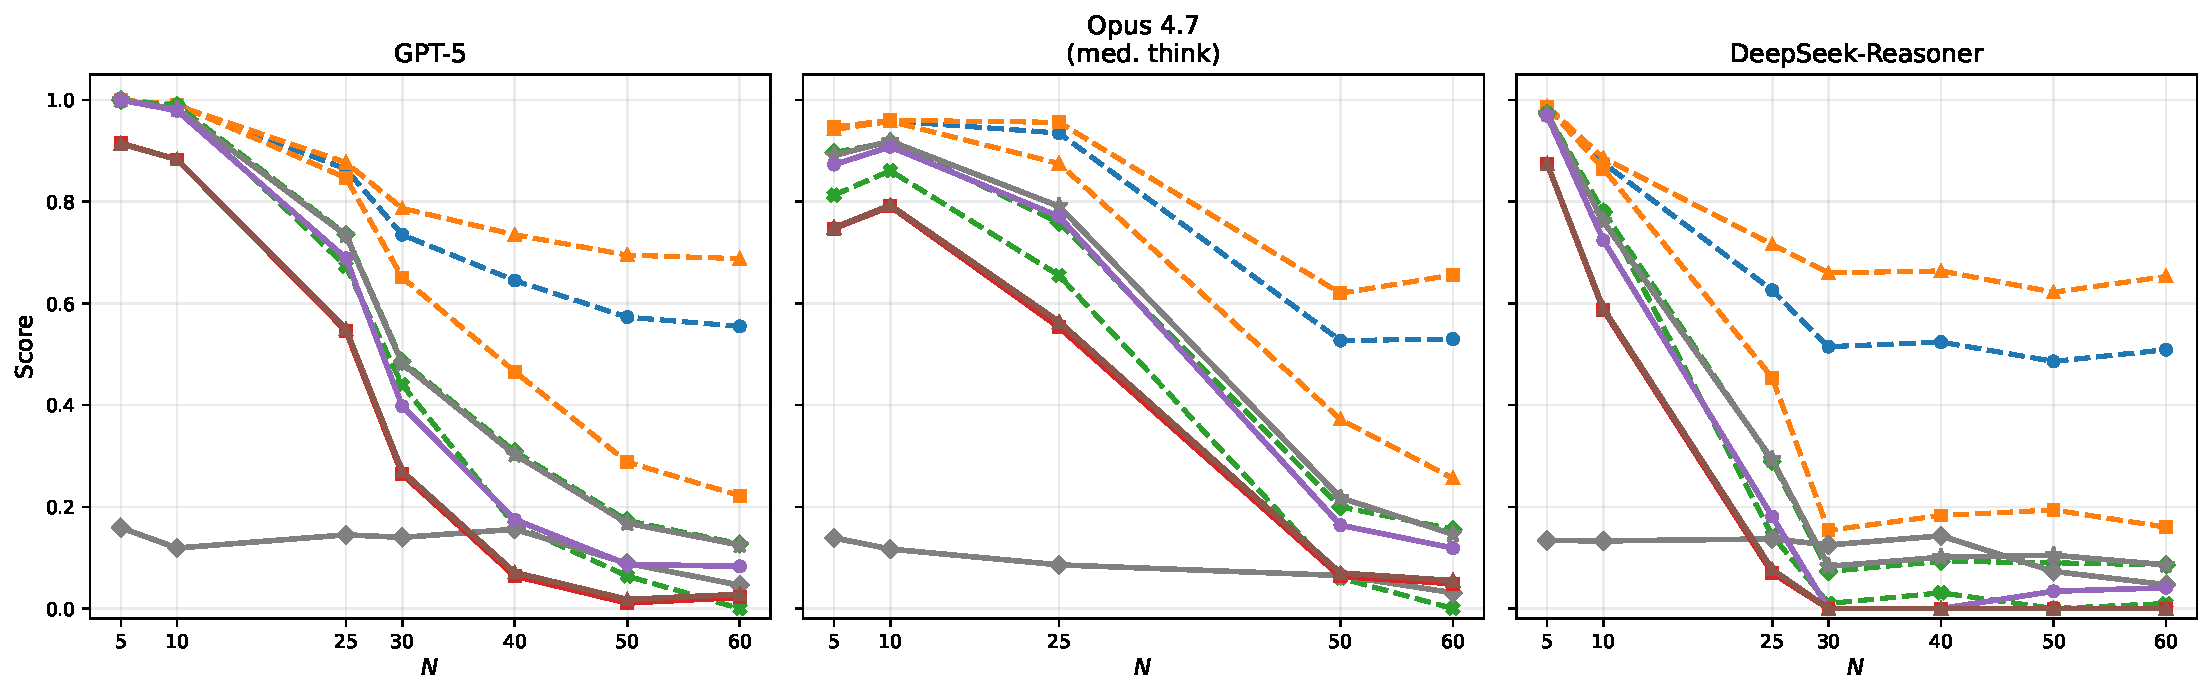
\includegraphics[width=\linewidth]
  {figures/shortcut_margin/fig_3sat_caseb_byN.pdf}
  \caption{Commercial 3-SAT.}
\end{subfigure}
\par\smallskip
\begin{subfigure}{0.94\textwidth}
  \centering
  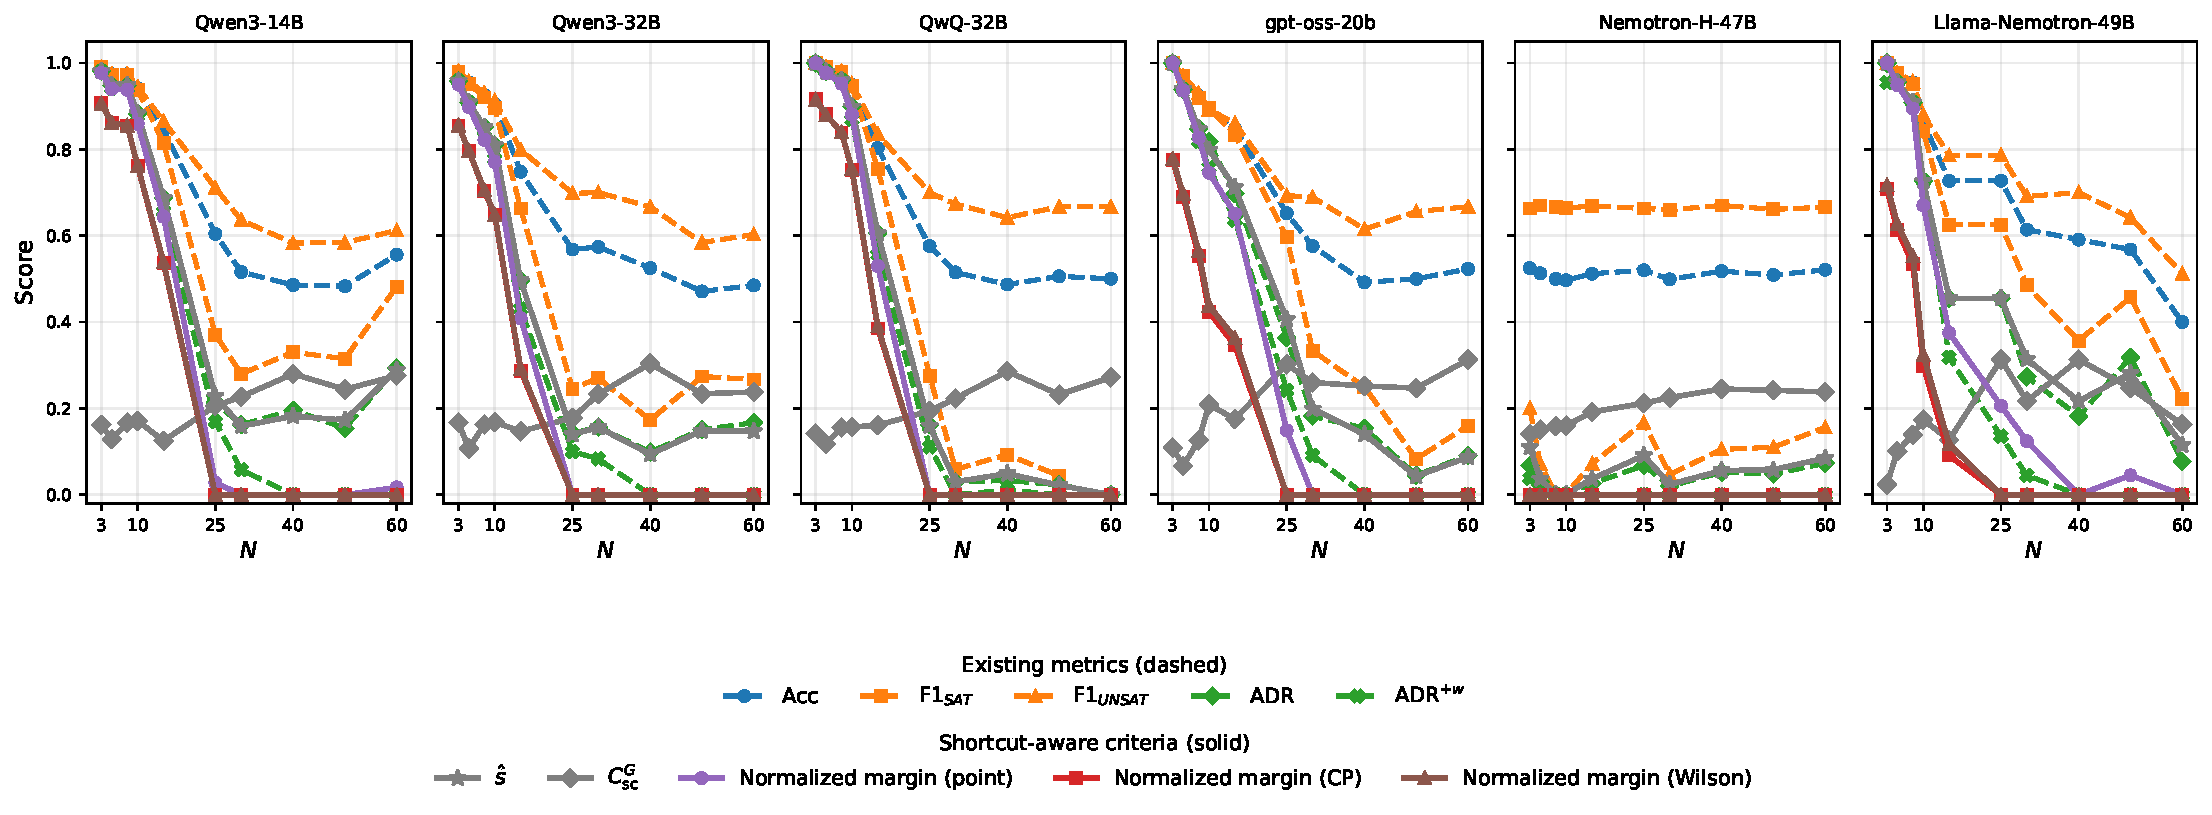
\includegraphics[width=\linewidth]
  {figures/shortcut_margin/fig_2sat_caseb_byN.pdf}
  \caption{Open-weight 2-SAT.}
\end{subfigure}
\caption{Shortcut-aware trajectories under the permutation-calibrated residual
shortcut ceiling. Conventional metrics often remain visibly nonzero after the
witness-grounded and confidence-bounded criteria have fallen sharply. Under
the No-Metrics interpretation, the separation is a claim gap: label agreement
persists after evidence of demonstrated constructive reasoning has weakened,
and the residual margin makes an additional design-conditional shortcut
charge.}
\Description{Two stacked sets of per-model line charts for commercial 3-SAT
and open-weight 2-SAT. Dashed accuracy and per-class F1 remain above the
witness-grounded ADR-plus-witness curve and the solid confidence-bounded
normalized-margin trajectories as instance size increases.}
\label{fig:no-metrics-caseb-trends}
\end{figure*}

\begin{figure*}[t]
\centering
\begin{subfigure}{0.94\textwidth}
  \centering
  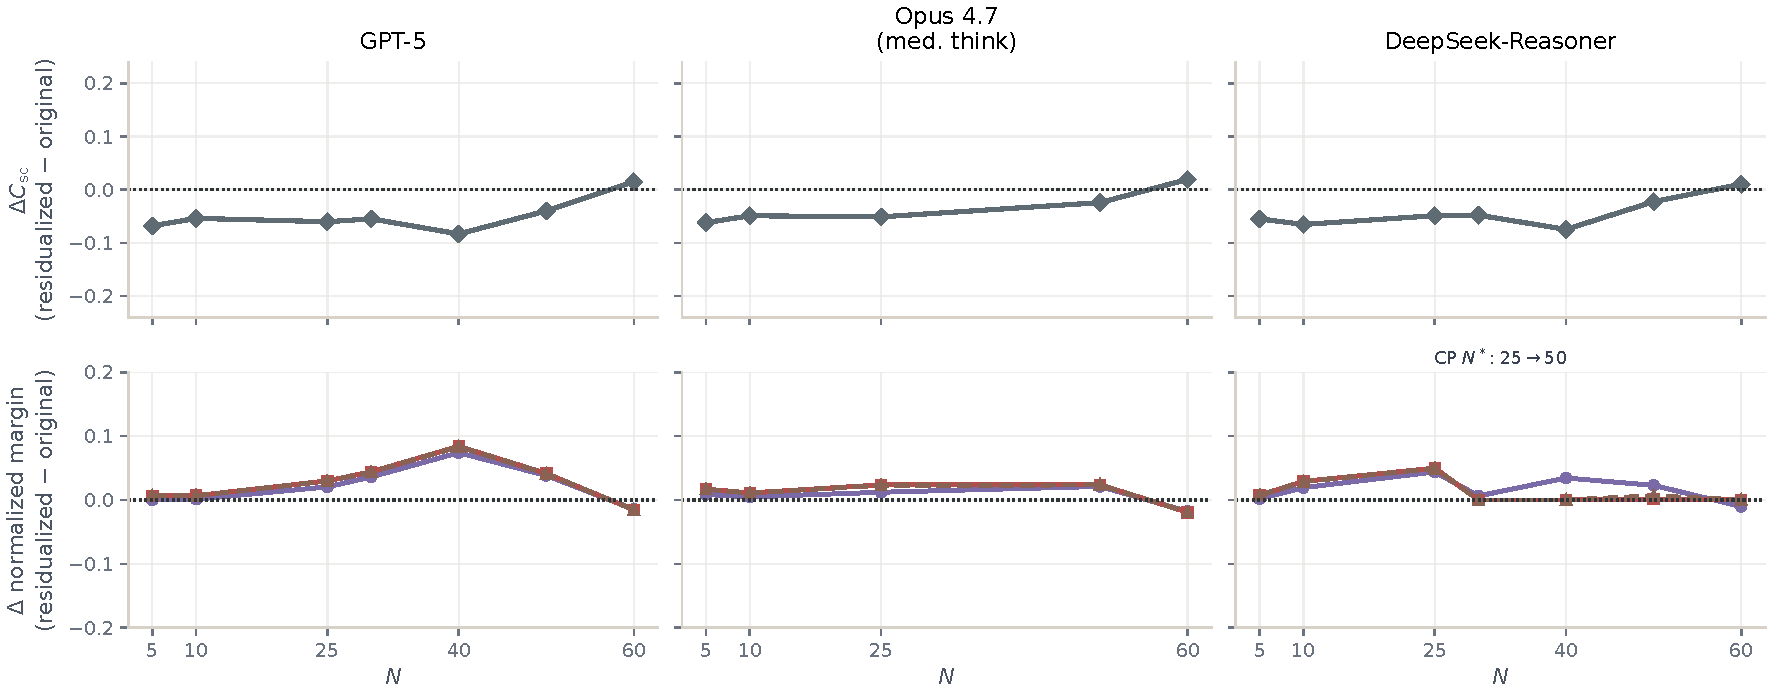
\includegraphics[width=\linewidth]
  {figures/shortcut_margin/fig_3sat_casec_byN.pdf}
  \caption{Commercial 3-SAT.}
\end{subfigure}
\par\smallskip
\begin{subfigure}{0.94\textwidth}
  \centering
  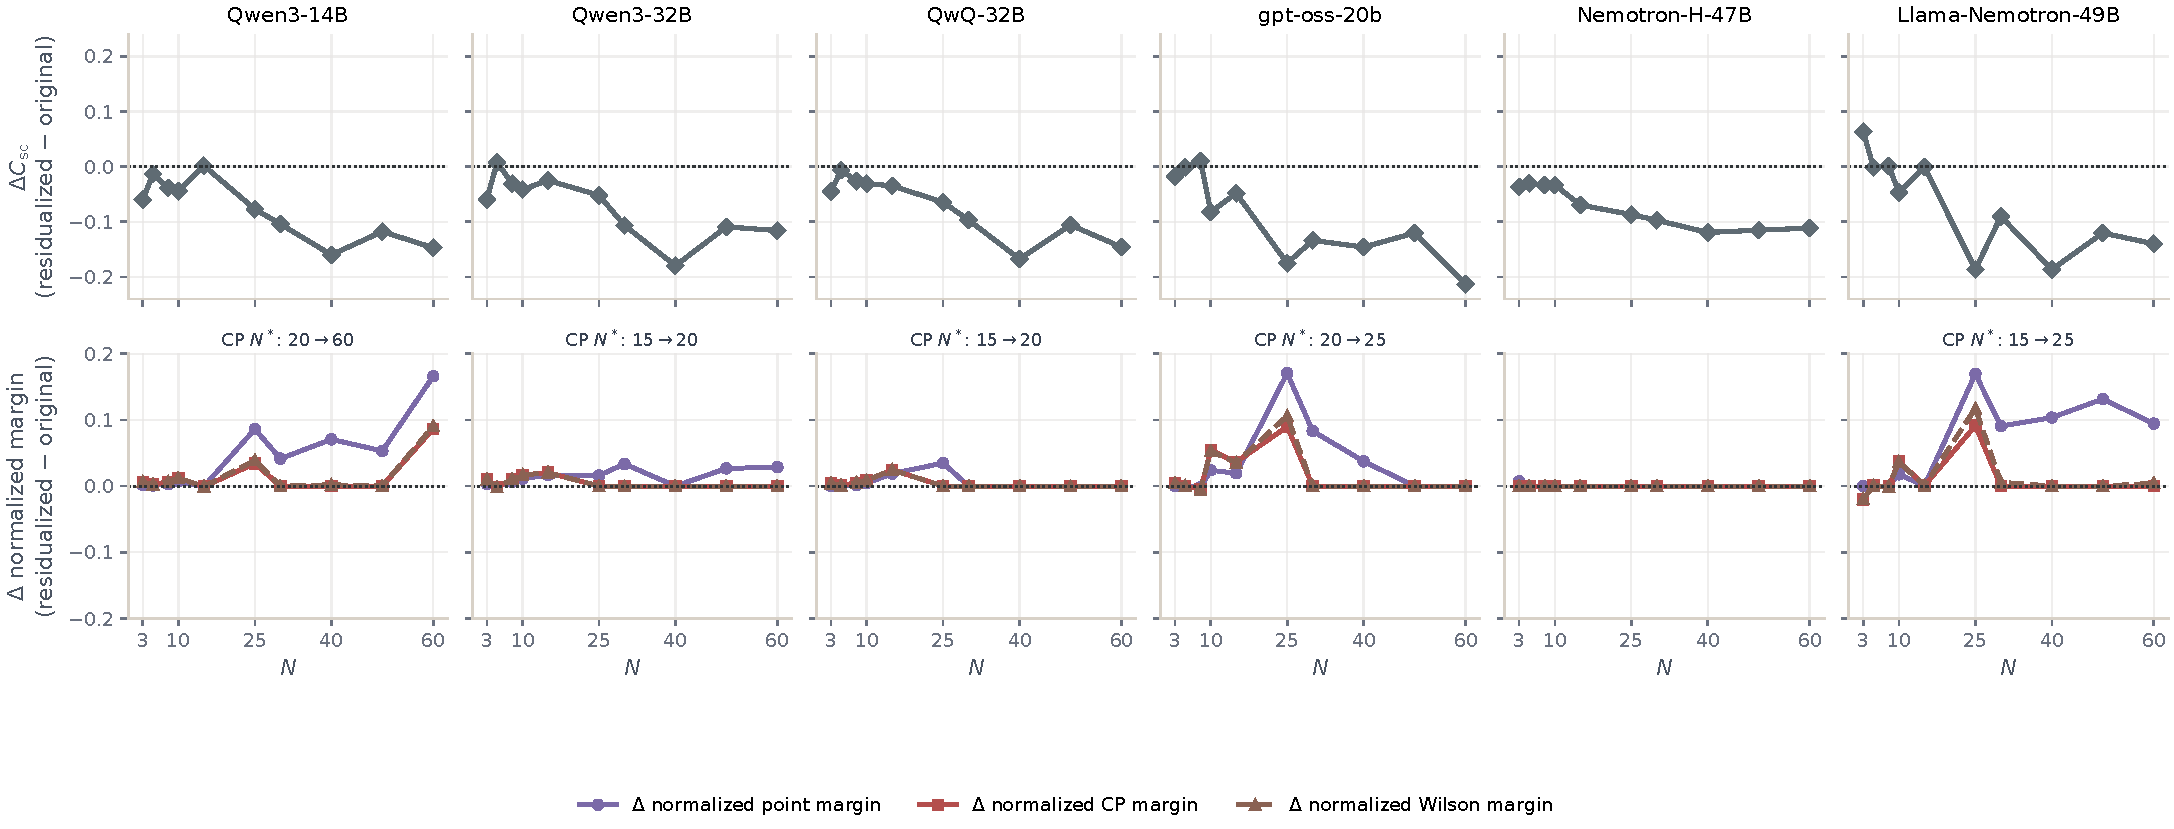
\includegraphics[width=\linewidth]
  {figures/shortcut_margin/fig_2sat_casec_byN.pdf}
  \caption{Open-weight 2-SAT.}
\end{subfigure}
\caption{Sensitivity of shortcut-aware conclusions to complexity
residualization. Each trajectory is the complexity-residualized specification
minus the original permutation-calibrated specification for the same frozen
model outputs. The upper row reports \(\Delta C_{\mathrm{sc}}\); the lower row
reports changes in normalized point, Clopper--Pearson, and Wilson margins.
Values above or below zero indicate that residualization respectively
increases or decreases the plotted quantity. Conventional metrics and
witness-grounded quantities are omitted because they are unchanged. CP
\(N^*\) annotations use the largest source-grid \(N\) with a strictly positive
full-precision signed CP margin; \(N=20\) is omitted from the 2-SAT
trajectories to match Fig.~\ref{fig:no-metrics-caseb-trends}. The figure
isolates nuisance-model sensitivity; it neither selects a universally correct
shortcut specification nor measures a change in latent reasoning ability.}
\Description{Two stacked sets of zero-centered per-model sensitivity charts
for commercial 3-SAT and open-weight 2-SAT. In each model column, the upper
panel plots the complexity-residualized minus original shortcut ceiling, and
the lower panel plots the corresponding changes in normalized point,
Clopper--Pearson, and Wilson margins. Horizontal zero lines distinguish
increases from decreases. Conventional metrics and witness curves are not
shown. Small labels identify changes in the positive-CP-margin boundary.}
\label{fig:no-metrics-casec-trends}
\end{figure*}

Together, the figures reinforce two conclusions from
Table~\ref{tab:representative-constraint-cases}. First, accuracy and per-class
F1 can remain moderate when \(\ADRw\), the closest machine-checkable proxy to
demonstrated reasoning in these archives, is small or zero. Second, a
shortcut-adjusted confidence margin answers a different, specification-bound
question: whether matched category behavior clears a stated nuisance ceiling.
Complexity residualization changes that ceiling and the resulting margins
without changing predictions or witnesses. The margin therefore neither
supersedes the witness nor identifies the model's internal mechanism.

\subsection{RQ2: Two-Sided Criteria Separate One-Sided, Label-Only, and Witness-Level Success}
\label{sec:constraint-rq2}

Matched two-sided summaries expose behavior that marginal metrics can obscure.
GPT-5 at 3-SAT \(N=60\) has positive-arm recall \(0.127\) and negative-arm
recall \(0.982\). Accuracy remains \(0.555\) and F1\(_-\) remains
\(0.688\), but \(\SepPoint=0.125\), \(\SepCP=0.067\), and
\(\ADRw=0\). The arm decomposition localizes the failure: the model retains
near-complete recognition of one category while losing the other. A large
per-class score on the easy arm cannot compensate in the product criterion.

The converse separation is equally important. A model can retain two-sided
\emph{label} discrimination without constructing a valid positive witness.
The graph-coloring rows in Table~\ref{tab:representative-constraint-cases}
show this directly. Llama-Nemo-49B at \(N=10\) has \(\SepCP=0.751\) but a
valid-coloring rate of only \(0.227\); Nemo-H-47B at \(N=8\) has
\(\SepCP=0.293\) but a valid-coloring rate of \(0.002\). The lower bound
therefore supports a claim about matched label recognition under the
constructed groups, not a claim about constructive graph reasoning. In these
rows, \(\ADRa\) is the more direct proxy for demonstrated reasoning because
the predicted coloring itself is checked against the graph constraints. The
large \(\SepCP-\ADRa\) gaps show that two-sided category recognition can remain
far from that constructive standard.

The 2-SAT follow-up strengthens this decomposition by adding evidence on the
UNSAT side. Table~\ref{tab:two-sided-witness} compares ordinary ADR,
positive-side witness ADR, and the follow-up-eligible two-sided witness audit.
Near-perfect label and SAT-witness results do not imply reliable production of
both artifacts. At \(N=3\), Qwen3-14B has \(\ADR=0.981\) and
\(\ADRw=0.981\), but \(\mathrm{ADR}^{+wu}=0.118\). At \(N=10\),
Qwen3-32B has \(\ADR=0.810\), \(\ADRw=0.777\), and
\(\mathrm{ADR}^{+wu}=0.281\). For gpt-oss-20b, the two-sided audit falls
from \(0.333\) at \(N=10\) to \(0\) at \(N=15\), even though the label-only
ADR remains \(0.545\) and the positive-side witness rate remains \(0.500\).

\begin{table*}[t]
\centering
\caption{Representative 2-SAT rows with the two-sided witness follow-up.
\(\mathrm{ADR}^{+wu}\) requires a verified SAT assignment and a verified
UNSAT clause subset and is computed only on follow-up-eligible pairs; it is
therefore reported as a separate audit rather than treated as an unconditional
lower bound on \(\ADRw\). \(\mathrm{ADR}^{+wu}_{\mathrm{all}}\) applies the
same two-sided requirement but uses every complete pair at that \(N\) as the
denominator, so pairs without a follow-up record count as failures; it is
computed by the group-analysis code on the current prediction files
(Section~\ref{sec:experimental-archives}), whereas the other columns are
archived values.}
\label{tab:two-sided-witness}
\renewcommand{\arraystretch}{1.08}
\resizebox{0.82\textwidth}{!}{%
\begin{tabular}{lrrrrrr}
\toprule
Model & \(N\) & ADR & \(\ADRw\) & \(\mathrm{ADR}^{+wu}\) & \(\SepCP\) &
\(\mathrm{ADR}^{+wu}_{\mathrm{all}}\)\\
\midrule
gpt-oss-20b (reason) & 3 & 1.000 & 1.000 & 0.818 & 0.976 & 0.273\\
Qwen3-14B (think) & 3 & 0.981 & 0.981 & 0.118 & 0.950 & 0.039\\
Qwen3-32B (think) & 10 & 0.810 & 0.777 & 0.281 & 0.753 & 0.066\\
gpt-oss-20b (reason) & 10 & 0.727 & 0.682 & 0.333 & 0.631 & 0.061\\
gpt-oss-20b (reason) & 15 & 0.545 & 0.500 & 0.000 & 0.485 & 0.000\\
QwQ-32B (think) & 20 & 0.283 & 0.242 & 0.231 & 0.222 & 0.030\\
\bottomrule
\end{tabular}%
}
\end{table*}

This follow-up does not by itself identify internal reasoning. A failure can
reflect inability to construct the requested artifact, an elicitation failure,
a parsing failure, or failure of the underlying reasoning process. Its value
is measurement separation: label discrimination, positive construction, and
available two-sided construction are empirically different observables and
should not be collapsed into one score. Among them, the verified two-sided
artifact is the strongest evidence that the model successfully externalized
the intended reasoning on that pair, although it remains an elicitation- and
protocol-dependent lower-bound-like proxy rather than a complete measure of
latent ability.

The choice between Clopper--Pearson and Wilson intervals is not the main source
of these gaps. Across the \(19\), \(59\), and \(45\) constraint rows, the mean
absolute difference \(|\SepCP-\SepWilson|\) is \(0.0043\), \(0.0050\), and
\(0.0040\), respectively; the maximum is \(0.011\) in every domain.
Agreement between the interval formulas strengthens the conclusion that a low
two-sided lower bound is not produced by one particular binomial
approximation. It does not identify the mechanism behind a high lower bound.

\subsection{RQ3: Controlled Conclusions Depend on Construction and Calibration}
\label{sec:constraint-rq3}

\paragraph{Pair matching.}
Pair rematching provides a direct test of construction dependence. The mean
\(\Dmatch\) is \(0.026\) on 3-SAT, \(0.023\) on 2-SAT, and \(0.072\) on
graph coloring. The maximum spreads are \(0.080\), \(0.182\), and \(0.364\).
For gpt-oss-20b at 2-SAT \(N=25\), the same predictions yield ADR values from
\(0.182\) to \(0.364\) under admissible rematchings. For QwQ-32B at graph
coloring \(N=40\), the range is \(0.155\) to \(0.436\). For
Llama-Nemo-49B at graph coloring \(N=60\), the original ADR and minimum ADR
are \(0\), whereas the maximum rematching reaches \(0.364\). The model
outputs are unchanged; only the construction of the controlled unit differs.

\paragraph{Group aggregation and repeated-success thresholds.}
\label{sec:group-adr-aggregation}

We apply the metrics in Section~\ref{sec:controlled-metrics:group} to the
current raw predictions for all three constraint domains. The analysis covers
three commercial 3-SAT configurations and six open-weight configurations for
each of 2-SAT and graph coloring. Table~\ref{tab:group-adr-overall} reports
the overall rows at \(\lambda=1\); the underlying analysis also exports every
model--size row, the full lambda sweep, group-level audit rows, completion
counts, and thresholds from one through ten successful pairs. The same
aggregation code also computes witness-aware counterparts (\(W\) and
\(A^{W}_{\ge k}\)) by calling each domain's established witness validator on
the positive-side response before crediting a pair, so the label-only and
witness-aware columns share pairs, groups, and denominators.

\begin{table*}[t]
\centering
\caption{Overall group-level results from the current raw predictions.
\(\mathrm{SGADR}=\mathrm{SGADR}_{1}\) and
\(\mathrm{SGADR}_{\star}=\mathrm{SGADR}_{\star,1}\). \(A_{\ge k}\) is the
fraction of evaluable groups containing at least \(k\) successful matched
pairs. GADR, ADR, SGADR, \(\mathrm{SGADR}_{\star}\), and \(A_{\ge k}\) are
label-only. \(W\) is the witness-aware pair rate on the same pairs with the
same denominator (\(\ADRw\) for SAT, \(\ADRa\) for graph coloring): a pair
counts only if both labels are correct and the positive-side response carries
a satisfying assignment or proper coloring verified by the domain's
established validator. \(A^{W}_{\ge k}\) is the fraction of evaluable groups
with at least \(k\) witness-verified successful pairs.}
\label{tab:group-adr-overall}
\renewcommand{\arraystretch}{1.04}
\resizebox{\textwidth}{!}{%
\begin{tabular}{llrrrrrrrrrr}
\toprule
Task & Model & GADR & ADR & \(W\) & SGADR & \(\mathrm{SGADR}_{\star}\) &
\(A_{\ge1}\) & \(A_{\ge5}\) & \(A_{\ge10}\) & \(A^{W}_{\ge1}\) & \(A^{W}_{\ge10}\)\\
\midrule
\multirow{3}{*}{3-SAT}
& GPT-5 & 0.539 & 0.526 & 0.452 & 0.421 & 0.276 & 0.942 & 0.507 & 0.203 & 0.768 & 0.188\\
& Opus 4.7 & 0.600 & 0.644 & 0.544 & 0.514 & 0.415 & 0.878 & 0.449 & 0.224 & 0.633 & 0.184\\
& DeepSeek-Reasoner & 0.342 & 0.350 & 0.289 & 0.249 & 0.123 & 0.771 & 0.286 & 0.171 & 0.486 & 0.171\\
\midrule
\multirow{6}{*}{2-SAT}
& Llama-Nemotron-Super-49B & 0.556 & 0.558 & 0.039 & 0.395 & 0.311 & 1.000 & 0.545 & 0.273 & 0.364 & 0.000\\
& Nemotron-H-47B & 0.038 & 0.038 & 0.004 & 0.017 & 0.001 & 0.147 & 0.029 & 0.001 & 0.010 & 0.000\\
& gpt-oss-20b & 0.540 & 0.551 & 0.485 & 0.423 & 0.303 & 0.903 & 0.613 & 0.258 & 0.742 & 0.258\\
& QwQ-32B & 0.460 & 0.464 & 0.218 & 0.397 & 0.215 & 0.701 & 0.485 & 0.340 & 0.598 & 0.010\\
& Qwen3-14B & 0.535 & 0.535 & 0.328 & 0.422 & 0.286 & 0.921 & 0.556 & 0.338 & 0.662 & 0.073\\
& Qwen3-32B & 0.453 & 0.455 & 0.235 & 0.338 & 0.207 & 0.884 & 0.455 & 0.248 & 0.653 & 0.008\\
\midrule
\multirow{6}{*}{Graph coloring}
& Llama-Nemotron-Super-49B & 0.318 & 0.318 & 0.062 & 0.192 & 0.101 & 0.839 & 0.258 & 0.065 & 0.258 & 0.000\\
& Nemotron-H-47B & 0.134 & 0.134 & 0.001 & 0.063 & 0.018 & 0.424 & 0.132 & 0.010 & 0.005 & 0.000\\
& QwQ-32B & 0.423 & 0.424 & 0.182 & 0.285 & 0.179 & 0.929 & 0.439 & 0.133 & 0.643 & 0.000\\
& Qwen3-14B & 0.320 & 0.320 & 0.165 & 0.184 & 0.102 & 0.797 & 0.349 & 0.050 & 0.456 & 0.000\\
& Qwen3-32B & 0.313 & 0.314 & 0.172 & 0.162 & 0.099 & 0.856 & 0.341 & 0.015 & 0.553 & 0.000\\
& gpt-oss-20b & 0.292 & 0.316 & 0.280 & 0.185 & 0.100 & 0.690 & 0.241 & 0.034 & 0.483 & 0.034\\
\bottomrule
\end{tabular}%
}
\end{table*}

Macro and micro weighting rarely drives the main conclusion in these data,
but it is not interchangeable. Across model--size slices, the mean absolute
gap \(|\mathrm{GADR}-\mathrm{ADR}|\) is \(0.0077\) on 3-SAT, \(0.0028\) on
2-SAT, and \(0.0014\) on graph coloring. The largest gaps are \(0.081\),
\(0.142\), and \(0.017\), respectively. Thus, equal-group and equal-pair
weighting usually agree because most groups contribute similar numbers of
complete pairs, but a single aggregate can still conceal a substantial
weighting decision in individual slices.

The nonlinear summaries reveal cross-group heterogeneity that pooled ADR does
not show. For Opus~4.7 on 3-SAT, GADR is \(0.600\),
while \(\mathrm{SGADR}_{1}=0.514\) and
\(\mathrm{SGADR}_{\star,1}=0.415\). For QwQ-32B on graph coloring, the same
sequence is \(0.423\), \(0.285\), and \(0.179\). QwQ-32B on 2-SAT has the
largest overall between-group variance, \(0.185\). These differences indicate that
moderate pair-level performance can be concentrated in some controlled
neighborhoods rather than sustained uniformly. The lambda sweep preserves
the identities in Equation~\eqref{eq:group-adr-lambda}; changing \(\lambda\)
changes the variance charge, not the underlying prediction record.

The repeated-success results provide the clearest test of stable behavior.
The largest overall \(A_{\ge10}\) is \(0.340\) at the precision shown in
Table~\ref{tab:group-adr-overall}, even though
\(A_{\ge1}\) is as high as \(1.000\). Across model--size slices,
\(A_{\ge10}=0\) in \(12/19\) 3-SAT rows, \(43/66\) 2-SAT rows, and
\(33/45\) graph-coloring rows. Qwen3-32B on graph coloring illustrates the
gap: ADR is \(0.314\), and \(85.6\%\) of evaluable groups contain at least
one successful pair, but only \(1.5\%\) contain ten. Qwen3-14B on 2-SAT has
GADR and ADR of \(0.535\), whereas \(A_{\ge10}=0.338\). Opus~4.7 reaches
ADR \(=0.644\) on 3-SAT, but only \(22.4\%\) of groups contain ten
successful pairs. Correct labels therefore occur much more often than
persistent success across variants of the same controlled construction.

This drop is consistent with the invariance motivation for group evaluation.
If a model had formed a stable representation of the decision-relevant
structure, incidental changes within the controlled neighborhood should not
turn most groups from success to failure. The observed threshold profiles do
not establish the opposite causal claim, because difficulty, correlated
errors, and missing outputs can also break consistency. Completion is high
for most overall rows, but ranges from \(0.711\) to nearly \(1\); an absolute
count threshold must therefore be reported with completion. The supported
conclusion is behavioral: isolated or sparse pair success overstates how
often the same model succeeds repeatedly within a group.

\paragraph{Group metrics versus witness evidence.}
Group consistency does not close the larger gap to witness-grounded
evidence. GADR, SGADR, and \(A_{\ge k}\) reuse the same label-pair outcomes as
ADR; none checks whether a SAT label is accompanied by a satisfying
assignment or whether a colorable label is accompanied by a valid coloring.
The witness-aware columns of Table~\ref{tab:group-adr-overall} apply the same
aggregation to the same groups after that check, so the distance between the
label-only and witness-aware columns is the part of group-level consistency
that was never witnessed. Four observations follow. Unless stated otherwise, the numbers below use the
\(130\) model--size slices.

\emph{Level.} \(W\) is below ADR in every overall row and every slice. Across
slices the ADR\(-W\) gap has mean \(0.171\) and median \(0.102\). Even in the
best-behaved rows the witness-verified share of label-pair successes is
\(0.83\)--\(0.89\) (GPT-5 \(0.86\), Opus~4.7 \(0.85\), DeepSeek-Reasoner
\(0.83\), gpt-oss-20b \(0.88\) on 2-SAT and \(0.89\) on graph coloring); in
the other graph-coloring rows it is \(0.00\)--\(0.55\), and Nemotron-H-47B
retains \(0.10\) on 2-SAT. Group weighting
does not help: GADR\(-W\) is within \(0.03\) of ADR\(-W\) in \(14/15\) rows,
because GADR and ADR agree on which pairs count and disagree only on how
groups are weighted.

\emph{Nonlinearity is not a witness check.} SGADR and
\(\mathrm{SGADR}_{\star}\) are numerically closer to \(W\) than ADR is in
\(105/130\) and \(102/130\) slices, and on 3-SAT all three overall SGADR
values fall slightly below \(W\) (\(-0.03\) to \(-0.04\)). This proximity is
coincidental. SGADR subtracts a within-group variance term, whereas \(W\)
removes pairs without a verified artifact; the two corrections respond to
different properties of the outputs. Accordingly, SGADR lands below \(W\) in
\(40/130\) slices, yet exceeds \(W\) by more than \(0.10\) in five overall
rows (Llama-Nemotron-Super-49B by \(0.36\) and QwQ-32B by \(0.18\) on 2-SAT;
Llama-Nemotron-Super-49B by \(0.13\), QwQ-32B and Qwen3-32B by \(0.10\)
elsewhere). A penalty for inconsistency cannot be read as a proxy for
demonstrated construction.

\emph{Ordering.} Ranking the six open-weight models by any label-only group
metric agrees with the ranking by \(W\) on only \(9\)--\(10\) of the \(15\)
model pairs on graph coloring, and on \(9\)--\(13\) of \(15\) on 2-SAT. The
repeated-success statistic is the least aligned: \(A_{\ge10}\) agrees with
\(W\) on \(9/15\) pairs in both domains. On 2-SAT, QwQ-32B has the largest
\(A_{\ge10}\) (\(0.340\)) but \(A^{W}_{\ge10}=0.010\), whereas gpt-oss-20b
retains its \(A_{\ge10}=0.258\) unchanged under the witness requirement.
Consistent label success across a group therefore neither implies nor orders
consistent witnessed success.

\emph{Thresholds.} The repeated-success rates degrade fastest.
\(A^{W}_{\ge10}\) is at most \(0.258\) and is \(0.000\) in five of the six
graph-coloring rows; \(A_{\ge10}>0\) in \(42\) slices, and in \(23\) of them
\(A^{W}_{\ge10}=0\). Sixty-five slices have \(A_{\ge1}=1.000\), yet their
\(A^{W}_{\ge1}\) ranges down to \(0.000\). Fifty-two slices have \(W=0\); in
\(50\) of them ADR, SGADR, and \(A_{\ge1}\) are all positive (GPT-5 at 3-SAT
\(N=60\): ADR \(0.127\), \(A_{\ge1}=0.700\), \(W=0\)). On 3-SAT, GPT-5 has \(A_{\ge1}=0.942\) but \(A^{W}_{\ge1}=0.768\),
and Opus~4.7 falls from \(A_{\ge10}=0.224\) to \(A^{W}_{\ge10}=0.184\).

In the source-separated witness analysis of RQ1, ADR already exceeds the
positive-side witness proxy in \(15/19\), \(47/59\), and \(40/45\) rows for
3-SAT, 2-SAT, and graph coloring. The group analysis sharpens that finding:
applying a group transformation to label outcomes cannot supply the missing
witness, and neither equal-group weighting, a variance penalty, nor a
repeated-success threshold moves a label-only summary reliably toward
\(W\). Group metrics measure persistence of label agreement within a
controlled construction; they remain summaries of predictions, not evidence
of the constructive ability that \(W\) checks. The stronger operational
target is therefore conjunctive: correct differentiation, persistence across
controlled variants, and a checkable witness where one exists. The current
group metrics measure the second property more directly than ordinary ADR,
while \(\ADRw\) and \(\ADRa\) remain closer to demonstrated reasoning because
they verify a semantic artifact. Neither alone identifies latent reasoning.


\paragraph{Reporting threshold.}
Table~\ref{tab:matched-threshold-boundaries} reports the matched-separability
prefix boundaries under four thresholds. GPT-5's 3-SAT boundary is \(25\),
\(30\), \(40\), or \(60\) when \(\tau\) is \(0.50\), \(0.25\),
\(0.10\), or \(0.05\). Qwen3-14B's 2-SAT boundary changes from \(15\) to
\(20\), \(50\), and \(50\) under the same sequence. These values answer
different effect-size questions; they are not competing estimates of a
threshold-free latent capability.

\begin{table*}[t]
\centering
\caption{Matched-separability prefix boundaries under alternative reporting
thresholds. Boundaries are comparable only within the same task family.}
\label{tab:matched-threshold-boundaries}
\renewcommand{\arraystretch}{1.08}
\resizebox{0.84\textwidth}{!}{%
\begin{tabular}{llrrrr}
\toprule
Domain & Model & \(N^*(0.50)\) & \(N^*(0.25)\) & \(N^*(0.10)\) & \(N^*(0.05)\)\\
\midrule
3-SAT & GPT-5 & 25 & 30 & 40 & 60\\
3-SAT & Opus 4.7 (med.\ think) & 25 & 25 & 50 & 60\\
3-SAT & DeepSeek-Reasoner & 10 & 10 & 25 & 25\\
\midrule
2-SAT & Qwen3-14B (think) & 15 & 20 & 50 & 50\\
2-SAT & Qwen3-32B (think) & 10 & 15 & 20 & 30\\
2-SAT & QwQ-32B (think) & 10 & 15 & 20 & 25\\
\bottomrule
\end{tabular}%
}
\end{table*}

\paragraph{Shortcut account and confidence requirement.}
Table~\ref{tab:shortcut-boundaries} summarizes the shortcut-margin archive. The
ideal and residual views use the same model outputs and lower-bound protocol;
they differ only in the charged ceiling. GPT-5's 3-SAT boundary changes from
\(30\) under \(\MarginZero\) to \(25\) under \(\MarginShortcut\). On 2-SAT,
Qwen3-32B changes from \(15\) to \(10\), gpt-oss-20b from \(20\) to \(15\),
and Llama-Nemotron-Super-49B from \(10\) to \(8\). Other SAT rows are
unchanged because the added shortcut charge does not cross a tested boundary.
We exclude the graph-coloring shortcut-ceiling contrast from this table: the
frozen runner invokes the same complexity-residualized configuration for the
files labeled as its raw and residualized branches, so those exports cannot
support a between-branch comparison. The matched-separability and witness
results for graph coloring remain usable because they come from the separate
archive and do not depend on that contrast.

\begin{table*}[t]
\centering
\caption{SAT shortcut-margin boundaries. \(N^*\) is the largest tested size with
a positive CP margin under the ideal \(0.25\) floor or the
permutation-calibrated residual shortcut ceiling. A dash denotes no positive
boundary in the reported grid. These are source-archive, design-conditional
boundaries rather than mechanism-independent capability estimates.}
\label{tab:shortcut-boundaries}
\renewcommand{\arraystretch}{1.08}
\resizebox{0.76\textwidth}{!}{%
\begin{tabular}{llrr}
\toprule
Domain & Model & \(\MarginZero\;N^*\) & \(\MarginShortcut\;N^*\)\\
\midrule
3-SAT & GPT-5 & 30 & 25\\
3-SAT & Opus 4.7 (med.\ think) & 25 & 25\\
3-SAT & DeepSeek-Reasoner & 10 & 10\\
\midrule
2-SAT & Qwen3-32B (think) & 15 & 10\\
2-SAT & gpt-oss-20b (reason) & 20 & 15\\
2-SAT & Nemotron-H-47B (r-on) & -- & --\\
2-SAT & Llama-Nemotron-Super-49B (r-on) & 10 & 8\\
\bottomrule
\end{tabular}%
}
\end{table*}

The lower-bound requirement can change the conclusion even before the shortcut
account changes. GPT-5 at 3-SAT \(N=40\) has an ideal point margin of
\(+0.053\), but its CP margin is \(-0.040\). gpt-oss-20b at 2-SAT \(N=25\)
has an ideal point margin of \(+0.156\), but its CP margin is \(-0.045\).
Thus a point estimate above a floor is not equivalent to a lower-bound claim.
The residual view adds another conditional choice: which feature battery is
admitted as a plausible shortcut class. Because the reported
\(\MarginShortcut\) ceiling is itself a calibrated point estimate, its positive
margins are best read as sensitivity results relative to the tested battery,
not as universal shortcut exclusion.

Together, RQ3 shows that controlled metrics correct specific weaknesses while
remaining design dependent. They prevent one arm from compensating for the
other, preserve matched structure, can require repeated pair success, and can
charge measured nuisance factors. Their numerical values and boundaries still
depend on the pairing rule, equal-group versus equal-pair weighting, the order
of nonlinear aggregation, the success-count threshold and effective group
size, the minimum reported effect size, the uncertainty construction, and the
stated adversary class. These dependencies are part of the evidence and must
be reported rather than hidden behind a single scalar.

\section{Discussion}

\paragraph{What the experiments establish.}
The experiments provide distinct empirical counterparts to the three formal
limitations. The witness-ordering reversals instantiate metric
non-monotonicity: better output performance under one criterion can accompany
worse performance under a stronger observable criterion. Pair-rematching,
threshold, and shortcut-ceiling sensitivity instantiate the design dependence
behind non-separability. None of these
analyses can empirically distinguish two models that produce exactly the same
outputs, which is precisely the mechanism non-identifiability of
Proposition~1.

\paragraph{What the experiments do not establish.}
The witness reference is asymmetric and incomplete, and controlled metrics do
not recover the latent pair
\((\delta_U,\epsilon_U)\). Accordingly, we do not interpret a lower
\(\SepCP\) as proof of weaker internal reasoning or a higher witness rate as a
complete reasoning score. The supported claims are conditional: better label
agreement, stronger two-sided matched behavior, more constructive
positive-side success, or greater robustness under a stated intervention.

\paragraph{A claim-matched reporting standard.}
A reasoning-oriented evaluation should report at least four layers of
evidence. First, conventional performance metrics describe deployment-facing
agreement. Second, arm-specific and controlled metrics expose one-sided and
local-contrast failures. Third, checkable witnesses or stronger task-specific
oracles validate outputs when available. Fourth, construction sensitivity,
nuisance-factor perturbations, and dependence-aware uncertainty delimit the
claim. A paper should state which layer supports each conclusion rather than
collapsing all layers into a single leaderboard number.

\paragraph{Applicability across model architectures.}
Our conclusions do not depend on a particular model architecture. They apply
to additive classifiers, attention-based models, graph neural networks, and
other systems whenever evaluation reduces model behavior to predictions or
scalar scores. These architectures differ in how they represent and combine
information, but this difference does not change the interpretation of the
resulting metric. A higher value establishes better performance under the
metric's observable criterion, not necessarily stronger reasoning.
Section~S6 of the supplementary material provides illustrative model-level
instantiations of this argument.

\paragraph{Metrics as summaries of interventions.}
Controlled metrics are best interpreted as summaries of model behavior under
particular interventions. Pair-level ADR summarizes whether predictions
change correctly across matched opposite-label instances. Group and cluster
metrics summarize whether this behavior remains consistent across related
variants. Metrics over semantics-preserving perturbations summarize
invariance to selected non-semantic changes. These measurements provide more
targeted evidence than evaluation on independently sampled instances, but
their interpretation depends on the quality of the interventions and the
aggregation rule. A higher controlled-metric value therefore indicates
stronger performance under the chosen intervention design, not necessarily
stronger reasoning ability.

The group results make this distinction observable
(Table~\ref{tab:group-adr-overall}). In \(88/130\)
model--size slices, no group contains ten successful matched pairs, although
many of the same slices contain isolated successes. Group evaluation therefore
reveals instability that pooled ADR can average away. Yet a model can also be
consistently right for a group-level non-semantic reason. Stable contrast
behavior should consequently be read alongside witness validity, rather than
as a replacement for it.

Intervention summaries become more informative when combined with
task-specific validation. In SAT solving, a satisfying assignment can
directly validate a positive answer. Controlled metrics summarize behavioral
consistency,
while witnesses test whether particular outputs satisfy stronger semantic
requirements. Neither should be treated as a universal standalone measure of
reasoning.

\subsection{Beyond Classification and Ranking Metrics}
\label{sec:discussion-output-metrics}

Although our formal development focuses on classification, ranking, and
controlled prediction metrics, the same underlying limitation applies more
broadly to output-based evaluation metrics. Many ML/LLM-based
software-engineering tasks are evaluated not by F1, MCC, or AUROC, but by
task-specific observable outcomes. For example, code-reasoning benchmarks may
use exact-match or pass@\(k\) metrics, while test-generation systems may be
evaluated by line or branch coverage. These metrics are appropriate for their
tasks, but they still summarize observable success rather than the mechanism
that produced it.

In a pass@\(k\) benchmark, the evaluator observes whether at least one of the
model's generated outputs is accepted by a checker. This is stronger than
unverified label agreement, because the output must satisfy a task-specific
correctness condition. However, the metric still does not reveal whether the
accepted output was produced by semantic reasoning, memorized patterns,
benchmark-specific cues, or lucky sampling. Similarly, coverage-based
test-generation metrics observe which lines or branches are executed by the
generated tests. Coverage is useful evidence about structural reachability,
but it does not by itself show that the generator understood the program's
intended behavior, produced meaningful assertions, or exposed the semantic
property of interest.

Thus, the limitation studied in this paper is not specific to a particular
metric formula. It arises whenever the evaluator observes only a finite
transcript of outputs and task-level success signals. Stronger checkers,
witnesses, and coverage measurements can make the observed success event more
meaningful, and they are often essential in practice. But unless the
evaluation also tests semantic sensitivity, side-channel invariance, or
mechanism-level evidence, output-based metrics alone cannot certify that
success came from reasoning.

Cohen's Kappa illustrates the same distinction. Kappa improves on raw
accuracy by correcting observed agreement for agreement expected from the
marginal class and prediction distributions. This makes it useful for
detecting cases where high accuracy is partly explained by class prevalence
or prediction bias. However, Kappa is still computed from the observable
confusion matrix. It does not reveal whether the agreements counted in the
confusion matrix were produced by semantic reasoning or by shortcut cues.
Thus, Kappa can improve the statistical interpretation of benchmark
agreement, but it does not solve the mechanism non-identifiability problem.

\paragraph{Broader use of prediction-output metrics.}
The concern studied in this paper is not unique to software-engineering
benchmarks. Surveys of deep-learning evaluation show that many of the same
families of metrics---accuracy, precision, recall, F1, ROC/AUC, error
metrics, ranking metrics, and task-specific output metrics---are widely used
across regression, classification, computer vision, natural-language
processing, and retrieval-augmented generation~\cite{Terven2025LossMetrics}.
This broader practice reinforces our point. These metrics are often useful
summaries of observable performance, and in many settings they are the
appropriate way to compare systems. Our claim is that when the intended
construct is reasoning ability, an output metric does not by itself establish
that the observed success was produced by semantic reasoning. The same
accuracy, ranking, coverage, or pass/fail signal may be compatible with
different underlying mechanisms. Software-engineering tasks make this issue
especially salient because semantic evidence, side-channel cues, and
benchmark artifacts can often be distinguished operationally through program
transformations, repairs, witnesses, or perturbations.

\section{Threats to Validity}
\label{sec:threats}

\paragraph{Secondary-analysis scope and archive versioning.}
The study reanalyzes frozen summary exports rather than rerunning models. This
prevents post-hoc prompt changes but limits us to the observables retained by
the source tables. Some overlapping shortcut-margin and matched-separability
rows differ slightly because
the archives reflect different reruns or parsing revisions. We mitigate this
threat by keeping the archives separate and by never combining row-level
values across versions. A final artifact should replace source filenames with
immutable commit hashes and include the raw per-instance predictions.

\paragraph{Witness asymmetry and elicitation.}
A satisfying assignment or valid coloring verifies constructive positive-side
success, but the supplied experiments do not require machine-checkable UNSAT
or non-colorability proofs. Witness failure can also arise from output format,
parsing, or instruction following. We therefore use witness success as a
stronger observable reference, not as a complete ground truth for reasoning.

\paragraph{Rounded values and post-hoc comparisons.}
The rank-discordance and sensitivity analyses use values rounded to three
decimals in the frozen tables. We exclude ties and do not infer hidden
precision, but a small number of orderings could change with full-precision
values. The analyses are also post-hoc. They should be replicated from
per-instance outputs with a preregistered comparison protocol.

\paragraph{Dependence and pseudo-replication.}
Matched examples share seed families, templates, and prompts. Per-arm
Clopper--Pearson and Wilson calculations use binomial assumptions that may be
optimistic under intra-group dependence. The source matched-pair protocol specifies a
matched-pair cluster bootstrap, but bootstrap replicates were not included in
the supplied summary exports. The present manuscript therefore reports the
available bounds and treats dependence-robust recomputation as required
before a final empirical claim.

\paragraph{Controlled-construction quality.}
Minimal edits can introduce lexical, syntactic, or structural artifacts, and
the shortcut feature set used by the residual ceiling is necessarily
incomplete. Pair rematching exposes one part of construction sensitivity but
does not enumerate every nuisance factor. A positive controlled result is
conditional on the stated intervention and shortcut audit.

\paragraph{Model, prompt, and domain coverage.}
The constraint tasks cover several model families, but they do not establish
universality across prompts, decoding settings, provider revisions, or
constraint generators. Boundaries are comparable only within a task family
and tested grid.


\section{Related Work}
\label{sec:related-work}

\subsection{Outcome-Based Evaluation of Reasoning-Oriented Tasks}
\label{sec:rw-outcome}

A large fraction of reasoning-oriented evaluation is ultimately based on
whether a model produces the correct final output. GSM8K, introduced by
Cobbe et al.~\cite{Cobbe2021GSM8K}, evaluates grade-school mathematical word
problems primarily through final-answer correctness; the same work trains
verifiers on candidate solutions whose supervision is determined by whether
the final numerical answer is correct. The MATH benchmark of Hendrycks et
al.~\cite{Hendrycks2021MATH} raises the difficulty substantially by using
competition mathematics problems and provides full step-by-step reference
solutions, but its standard benchmark comparison is still based primarily on
normalized final-answer accuracy. GPQA~\cite{Rein2024GPQA} similarly improves
the quality of the evaluation task by using expert-authored graduate-level
science questions that remain difficult for skilled non-experts even with web
access. These benchmarks differ substantially in domain, difficulty, and data
construction, but they exemplify a common evaluation pattern: a task is chosen
because successful completion plausibly requires reasoning, while the reported
score is determined mainly by the correctness of the final answer.

Such outcome metrics are valuable measures of task success. A higher GSM8K,
MATH, or GPQA accuracy establishes that a system answers more benchmark items
correctly under the evaluated protocol. It does not, however, identify the
mechanism responsible for those correct answers. Correct outputs may be
compatible with valid multi-step reasoning, memorized knowledge, retrieval,
elimination strategies, shortcut cues, search-and-selection effects, or
combinations of these mechanisms. Our work therefore does not dispute the
validity of final-answer metrics for their immediate behavioral criterion.
Instead, it studies the additional inferential step from better outcome
performance to a claim of stronger reasoning ability.


\subsection{Reasoning-Trace and Process Evaluation}
\label{sec:rw-trace}

A second line of work evaluates the generated reasoning process rather than
only the final answer. ROSCOE~\cite{Golovneva2023ROSCOE} introduces a suite of
automatic metrics for step-by-step rationales, including dimensions related
to semantic alignment, semantic similarity, logical consistency,
informativeness, factuality, and language quality. ReCEval~\cite{Prasad2023ReCEval}
views a generated reasoning chain as an informal proof and evaluates two
properties: correctness, including whether intermediate conclusions are
supported and non-contradictory, and informativeness, including whether a step
adds information useful for deriving the generated answer. ReCEval implements
these ideas using natural-language-inference models and
$\mathcal{V}$-information. These approaches provide strictly richer observable
evidence than final-answer accuracy because they can distinguish reasoning
traces that reach the same answer but differ in detectable intermediate
errors.

Related work on process supervision makes the same distinction from the
training perspective. Lightman et al.~\cite{Lightman2024Verify} compare
outcome supervision, which labels a complete solution by its final result,
with process supervision, which provides feedback on intermediate steps, and
show that process supervision can substantially improve performance on MATH.
This line of work demonstrates that intermediate-step evidence is useful and
that final-answer supervision is not the only way to evaluate or train
reasoning systems.

However, observable trace quality and mechanism faithfulness are distinct
claims. Turpin et al.~\cite{Turpin2023UnfaithfulCoT} show that chain-of-thought
explanations can systematically rationalize answers influenced by hidden
biasing features without reporting those influences. Lanham et
al.~\cite{Lanham2023Faithfulness} evaluate faithfulness by intervening on
chain-of-thought traces and find substantial task- and model-dependent
variation in how strongly answers depend on the stated reasoning. Thus, a
high-quality rationale under ROSCOE, ReCEval, or a learned verifier is stronger
evidence than final-answer correctness, but it does not by itself establish
that the visible rationale is the causal mechanism that produced the answer.

This distinction is important for our analysis. Our formal results focus on
prediction- and score-based metrics, while trace evaluators illustrate how
richer observations can narrow, but not automatically eliminate, the gap
between observable behavior and latent reasoning mechanisms.


\subsection{Benchmark Reliability, Construct Validity, and Reasoning Claims}
\label{sec:rw-validity}

Recent work has increasingly treated reasoning evaluation as a measurement
and validity problem rather than only a metric-selection problem. Salaudeen et
al.~\cite{Salaudeen2025Validity} distinguish measurement instruments,
measurements, evaluations, and claims, and argue that validity depends on
whether the available evidence supports the particular claim being made.
Their framework separates directly measurable criteria from broader latent
constructs such as reasoning and emphasizes that increasingly broad capability
claims require increasingly strong forms of validity evidence. Bean et
al.~\cite{Bean2025ConstructValidity} provide complementary empirical evidence
through a systematic review of 445 LLM benchmarks. They analyze how target
phenomena are operationalized through tasks and metrics and identify recurring
construct-validity weaknesses in benchmark definition, sampling, scoring, and
claim interpretation.

Most directly related to the empirical motivation of our work, Mousavi et
al.~\cite{Mousavi2025Garbage} systematically audit SocialIQA, ToMi, and
FauxPas-EAI and identify structural, semantic, and pragmatic problems in both
benchmark items and evaluation protocols. Their re-evaluations show that
scores can change materially after data cleaning, context changes, semantic
rephrasing, and alternative scoring, without any corresponding change in the
underlying model parameters. Their findings demonstrate that a benchmark score
is a property of the broader evaluation pipeline, not a context-free measure
of a model's reasoning ability, and that high scores may partly reflect
format-specific regularities rather than stable inference from the intended
information.

Our work is complementary to these validity-centered studies. Salaudeen et
al. provide a general framework for asking what claims an evaluation can
support, Bean et al. document how construct-validity problems arise in current
benchmark practice, and Mousavi et al. show empirically how benchmark and
protocol defects can distort reasoning scores. We study a narrower but more
formal identification problem: even when benchmark labels and scoring
procedures are taken as correct, finite prediction or score observations do
not in general identify whether success was produced by semantic reasoning or
by a non-semantic shortcut, and metric-based model rankings need not be
monotone in reasoning ability. In this sense, benchmark cleaning and better
construct operationalization address important sources of invalidity, but do
not by themselves resolve mechanism non-identifiability.

Prior surveys of classification metrics, such as Naidu et
al.~\cite{Naidu2023ReviewMetrics}, address a different problem: selecting and
standardizing statistical metrics for particular prediction settings. Our
focus is not on identifying a universally preferable confusion-matrix or
ranking metric. Rather, we ask what reasoning-oriented claims can be supported
from the observable information retained by such metrics.


\subsection{Controlled, Contrastive, and Intervention-Based Evaluation}
\label{sec:rw-controlled}

A complementary strategy strengthens the evaluation design rather than only
changing the scoring formula. Contrast sets perturb test instances in small
but meaningful ways, often changing the gold label, to probe local decision
boundaries and expose systematic gaps in standard test
sets~\cite{Gardner2020ContrastSets}. CheckList applies behavioral testing
through capabilities, invariance tests, and directional expectation
tests~\cite{Ribeiro2020CheckList}. Metamorphic testing similarly specifies
relations among multiple executions when a simple oracle is
unavailable~\cite{Chen2018MetamorphicSurvey}. These approaches share an
important principle: evidence about a model becomes more informative when its
behavior is evaluated under controlled changes rather than on isolated,
independently sampled inputs.

Recent software-engineering evaluations instantiate this principle directly.
Ding et al.~\cite{VDCL:Ding:2024} use vulnerability-related paired evaluation
to test whether code models distinguish closely related programs with
different vulnerability labels. In satisfiability solving, Zhang et
al.~\cite{Zhang2026SAT} introduce Accurate Differentiation Ratio (ADR) to
measure whether a model correctly distinguishes matched SAT/UNSAT formulas.
Such controlled metrics are closer to the intended semantic relation than
marginal accuracy when the pairs are well constructed. They can suppress
strategies that succeed only from class imbalance or cues shared within a
pair.

Our work analyzes the remaining boundary of this approach. A controlled
metric is still a metric over a particular intervention design. Label-changing
edits may introduce residual artifacts, semantics-preserving transformations
may fail to cover all nuisance factors, and repeated group or cluster success
may remain correlated through shared shortcuts. We therefore distinguish the
\emph{design} of a semantic-changing or semantics-preserving intervention from
the \emph{metric} that aggregates its outcomes. ADR, group ADR, and cluster
metrics provide stronger behavioral evidence than marginal prediction
metrics, but the observed success can still combine semantic success with
residual shortcut or guessing success. This motivates the non-separability
analysis developed in this paper.


\subsection{Explanation-Based and Mechanism-Oriented Evidence}
\label{sec:rw-explanation}

Post-hoc explanation methods provide another source of evidence about why a
model predicts as it does. For graph neural networks, GNNExplainer searches
for a subgraph and feature subset that approximately preserve a model's
prediction~\cite{Ying2019GNNExplainer}. Integrated Gradients, SHAP, and
DeepLIFT estimate feature or token contributions using gradients,
perturbations, or reference activations~\cite{Sundararajan2017IG,
LundbergLee2017SHAP,Shrikumar2017DeepLIFT}. Such methods can help diagnose
whether a model appears to rely on vulnerability-relevant program structure,
formula semantics, identifier names, API names, formatting, or other
side-channel cues.

Explanation methods are complementary to prediction metrics because they
retain or recover information that a scalar performance score discards. At
the same time, an explanation must itself be validated: different explanation
methods can allocate influence differently, and evidence that a feature
influenced a prediction is not the same as evidence that the feature is
semantically valid for the intended task. For this reason, explanations are
most useful in our framework when they motivate controlled interventions. If
an attribution highlights a suspected side-channel factor, changing that
factor while preserving task semantics provides a direct behavioral test of
whether the prediction depends on it. Conversely, modifying the
label-determining semantic relation while holding nuisance factors fixed tests
semantic sensitivity.


\subsection{Positioning of This Work}
\label{sec:rw-positioning}

The preceding literature progressively enriches the evidence used to evaluate
reasoning: outcome benchmarks measure final task success; trace metrics and
process supervision inspect intermediate rationales; validity-centered work
examines the connection between measurements and capability claims; and
contrastive, metamorphic, and explanation-based methods probe model behavior
under more informative designs. Our contribution is to characterize a common
identification and validity boundary across these perspectives. We formalize
why finite prediction and score observations do not, without additional
assumptions, uniquely identify the mechanism responsible for benchmark
success or guarantee that metric ordering is an ordering of reasoning
ability. We further analyze why controlled pair, group, and cluster metrics
reduce some shortcut opportunities without fully separating semantic success
from residual non-semantic success.

Accordingly, the conclusion of this work is not that reasoning metrics are
useless. Different metrics are valid for different observable criteria, and
richer evaluation designs support stronger behavioral claims. The central
question is instead how far those claims may be extended. We use checkable SAT
witnesses, controlled interventions, and nuisance-factor audits to study how
additional information narrows
the gap between benchmark performance and reasoning claims. This places our
work between metric analysis and construct-validity analysis: we treat
metrics as useful summaries of observable behavior while making explicit the
additional assumptions and evidence required to interpret those summaries as
evidence of reasoning.



\section{Conclusion}
\label{sec:conclusion}

This paper distinguishes the observable criterion computed by an evaluation
metric from the broader construct of reasoning ability. Metrics based on
finite labels, predictions, or scalar scores cannot in general identify the
mechanism that produced success. Their values need not be monotone in
semantic reasoning, and controlled-success probabilities do not uniquely
separate semantic from residual non-semantic success.

The empirical reanalysis shows that these are practical, not merely
philosophical, boundaries. Conventional metrics remain nontrivial after
constructive witness production collapses; model orderings reverse relative
to witness-aware evidence; and controlled results change under pair
rematching, effect thresholds, confidence
requirements, and shortcut-ceiling specifications. Matched and
confidence-bounded metrics are valuable precisely because they expose some of
these failures. Group analysis adds a further boundary: no group reaches ten
successful matched pairs in \(88/130\) model--size slices, even though
isolated pair success is common. These metrics still measure behavior under a
selected design rather than a design-independent latent mechanism.

The appropriate conclusion is therefore not that reasoning evaluation is
impossible or that metrics are useless. It is that claim strength must track
evidence strength. Accuracy and F1 support claims about benchmark agreement.
ADR and matched separability support claims about controlled contrast
behavior. Group thresholds support claims about persistence across controlled
variants. Checkable witnesses support constructive correctness claims and are
the closest machine-checkable proxy to demonstrated reasoning in the
constraint archives. Perturbations and nuisance-factor audits support
conditional invariance claims. Stronger claims about reasoning require these
sources of evidence to be combined and their remaining assumptions made
explicit.


%%
%% The next two lines define the bibliography style to be used, and
%% the bibliography file.
\bibliographystyle{ACM-Reference-Format}
\bibliography{paper}


\end{document}
\endinput
%%
%% End of file `sample-acmsmall-conf.tex'.
